\documentclass[12pt, a4paper]{article}

\usepackage[top=2.5cm, bottom=2.5cm, left=3cm, right=3cm]{geometry}
\usepackage{mdframed}
\usepackage[utf8]{inputenc}
\usepackage[T1]{fontenc}
\usepackage[spanish,es-nodecimaldot]{babel}
\usepackage{amsmath}
\usepackage{float}
\usepackage[margin=10pt, font=small, labelfont=bf]{caption}
\usepackage{booktabs}
\usepackage{graphicx}
\usepackage{xcolor}
\usepackage{hyperref}
\usepackage{natbib}
\usepackage{longtable}
\usepackage{comment}
\usepackage{setspace}
\usepackage{titlesec}
\usepackage{fancyhdr}
\usepackage{tabularx}
\usepackage{array}
\usepackage{enumitem}
\usepackage{microtype}
\usepackage{tikz}
\usepackage{graphicx}
\usepackage{float}
\usetikzlibrary{positioning, arrows.meta, shapes.geometric}

\setlength{\textfloatsep}{18pt plus 2pt minus 4pt}
\setlength{\floatsep}{12pt plus 2pt minus 2pt}
\setlength{\intextsep}{14pt plus 2pt minus 2pt}
\setstretch{1.15}
\setlength{\parindent}{0pt}
\setlength{\parskip}{8pt}
\setlist[itemize]{leftmargin=1.25em,itemsep=2pt,topsep=3pt}
\renewcommand{\arraystretch}{1.18}

\titleformat{\section}
  {\large\bfseries}{\thesection.}{0.5em}{}
  [\vspace{2pt}\hrule\vspace{4pt}]
\titleformat{\subsection}
  {\normalsize\bfseries}{\thesubsection.}{0.5em}{}
\titlespacing{\section}{0pt}{18pt}{8pt}
\titlespacing{\subsection}{0pt}{14pt}{6pt}

\hypersetup{colorlinks=true, linkcolor=blue!60!black, citecolor=blue!60!black, urlcolor=blue!60!black}

\pagestyle{fancy}
\fancyhf{}
\fancyhead[L]{\footnotesize Centro Javeriano de Competitividad}
\fancyhead[R]{\footnotesize \reportnumber}
\cfoot{\thepage}
\setlength{\headheight}{14pt}
\renewcommand{\headrulewidth}{0.4pt}

\geometry{margin=1in}
\graphicspath{{figures/}}
\newcommand{\figurelang}{es}
\newcommand{\reportseries}{Informes sobre la Productividad en Colombia}
\newcommand{\reportseriesdesc}{Evidencia para entender y fomentar la productividad}
\newcommand{\reportnumber}{Informe 03}
\newcommand{\reporttitle}{Inteligencia Artificial y Empleo en Colombia}
\newcommand{\reportsubtitle}{Exposición, complementariedad y transformación del trabajo}
\newcommand{\reportauthorone}{Oliver Pardo}
\newcommand{\reportauthoroneaffil}{Profesor asociado del Departamento de Administración, Pontificia Universidad Javeriana y director del Centro Javeriano de Competitividad}
\newcommand{\reportauthortwo}{Jorge Orozco}
\newcommand{\reportauthortwoaffil}{Consultor de investigación del Centro Javeriano de Competitividad, Pontificia Universidad Javeriana}
\renewcommand{\contentsname}{Tabla de contenido}

\title{\reporttitle\\\reportsubtitle}
\author{\reportauthorone \and \reportauthortwo}
\date{Julio de 2026}

\begin{document}

\begin{titlepage}
\thispagestyle{empty}
\vspace*{0.6cm}

\begin{center}

\includegraphics[width=0.58\textwidth]{logo_cjc_palatino_horizontal.png}
\end{center}

\vspace{1.5cm}

\begin{center}
{\Large\bfseries \reportseries\par}
\vspace{0.15cm}
{\large \reportseriesdesc\par}

\vspace{1.4cm}

{\large\bfseries \reportnumber\par}
\vspace{0.45cm}
{\Huge\bfseries \reporttitle\par}
\vspace{0.35cm}
%{\Large \reportsubtitle\par}
%\vspace{0.65cm}
{\large\bfseries \reportauthorone\par}
{\normalsize \reportauthoroneaffil\par}
\vspace{0.25cm}
{\large\bfseries \reportauthortwo\par}
{\normalsize \reportauthortwoaffil\par}
\end{center}

\vfill

\begin{center}
{\large Septiembre de 2026\par}
\end{center}

\end{titlepage}

\begin{mdframed}[
  linewidth=1pt,
  linecolor=gray!60,
  backgroundcolor=gray!6,
  innertopmargin=12pt,
  innerbottommargin=12pt,
  innerleftmargin=14pt,
  innerrightmargin=14pt
]
\section*{Resumen ejecutivo}
\addcontentsline{toc}{section}{Resumen ejecutivo}

La inteligencia artificial (IA) está automatizando al menos algunas de las tareas realizadas por los trabajadores. Este informe estudia cómo esa transformación puede afectar al empleo colombiano a partir de dos dimensiones. La primera es qué tan expuestas están las ocupaciones a ser afectadas por la IA. La segunda es si esta exposición se traduce en que la IA complementa las tareas del trabajador o si por el contrario las sustituye.

El 25\% del empleo colombiano presenta algún grado de exposición y el 8,0\% se ubica en niveles altos o muy altos. La exposición aumenta con el ingreso y la educación, es mayor entre mujeres y trabajadores formales y se concentra especialmente en actividades financieras, información y comunicaciones. Oficinistas, contadores, empleados de centros de llamadas, auxiliares contables, secretarios y desarrolladores de software aparecen entre las ocupaciones de alta exposición con mayor peso en el empleo.

Los trabajadores de mayores ingresos están más expuestos, pero también se concentran en ocupaciones donde las características del trabajo favorecen una relación más complementaria con la IA. La razón entre empleo en ocupaciones de alta y baja complementariedad pasa de 0,75 en el primer quintil de ingreso a 2,80 en el quinto. También se observan diferencias por educación, género y formalidad. La distribución de las ganancias potenciales de la inteligencia artificial depende, por tanto, no solo de quién está expuesto, sino también del tipo de tareas que realiza y de su capacidad para reorganizarlas alrededor de la nueva tecnología.

%La evidencia internacional muestra por qué esta distinción importa. El uso de inteligencia artificial ha producido aumentos de productividad en centros de llamadas, desarrollo de software, consultoría y escritura, pero también existen señales de menor demanda laboral en algunos mercados altamente expuestos.
El reto para Colombia consiste en facilitar la adopción de la IA y el rediseño de tareas allí donde la tecnología pueda complementar al trabajador. Al mismo tiempo, el país debe fortalecer las capacidades de quienes se encuentran en ocupaciones con alta posibilidad de sustitución para transitar hacia otras ocupaciones. El presente informe ayuda a identificar hacia qué ocupaciones deben orientarse estos esfuerzos.

\end{mdframed}

\newpage
\tableofcontents
\newpage

\section{Introducción}

La IA está ampliando la frontera de lo que puede ser automatizado. A diferencia de olas anteriores de cambio tecnológico, que afectaron principalmente tareas rutinarias y codificables, los nuevos sistemas pueden producir textos, resumir documentos, generar código, analizar información y apoyar procesos de decisión. La transformación tecnológica alcanza así con mayor intensidad a ocupaciones administrativas, profesionales y relativamente calificadas.

No obstante, el efecto de la IA sobre los trabajadores puede ser positivo o negativo dependiendo de qué tanto las tareas realizadas por la IA complementan o sustituyen las tareas que quedan en manos del trabajador. Si las complementan, el trabajador genera más valor agregado gracias a la IA, lo que puede contribuir a mantener su puesto de trabajo y elevar su salario. Si las sustituyen, las empresas pueden prescindir de estos trabajadores y presionar a la baja los salarios.

%El efecto sobre el mercado laboral depende, sin embargo, de algo más que las capacidades técnicas de estas herramientas. Una empresa puede utilizarlas para reducir el tiempo requerido por una tarea, mejorar su calidad, ampliar la producción o reasignar trabajadores hacia actividades de mayor valor. También puede automatizar tareas y reducir la cantidad de trabajo necesaria para producir un mismo resultado. La adopción, la organización del trabajo, las habilidades de los trabajadores y la respuesta de la demanda determinan qué trayectoria termina predominando.

Este informe evalúa el impacto de la IA sobre los trabajadores colombianos. En primer lugar se mide, para cada ocupación reportada en la Gran Encuesta Integrada de Hogares (GEIH), la \textit{exposición}: la magnitud en que las tareas asociadas a la ocupación pueden ser automatizadas por la IA. En segundo lugar se mide la \textit{complementariedad}: en qué medida la IA complementa al trabajo humano en lugar de sustituirlo. Para la medición de la exposición se usa el índice de exposición a la IA desarrollado por la Organización Internacional del Trabajo (OIT) y el Instituto Nacional de Investigación (NASK) de Polonia documentado por \citep{gmyrek2025}. Para la medición de la complementariedad se utiliza la metodología desarrollada por \citet{felten2021} y \citet{pizzinelli2023}. A partir de esta información se infiere cómo la IA afectará potencialmente a distintos géneros, logros educativos y niveles de ingreso.

%El interés no está únicamente en identificar dónde puede producirse una transformación más intensa de las tareas, sino también en entender dónde existen mejores condiciones para convertir ese cambio tecnológico en aumentos de productividad y dónde pueden surgir transiciones laborales más complejas.

\section{Indicadores de exposición y complementariedad}

\subsection{Indicador de exposición}

El primer indicador proviene de la actualización de 2025 del índice de exposición ocupacional a la IA elaborado por la OIT y NASK \citep{gmyrek2025}. Su unidad de análisis es la tarea. Cada tarea recibe un puntaje entre cero y uno según la capacidad de la IA para realizarla. El puntaje de una ocupación corresponde al promedio de los puntajes de las tareas que realiza la ocupación. Un mayor valor indica que las tareas realizadas por la ocupación pueden ser realizadas por la IA. A partir de estos puntajes, el presente informe clasifica a las ocupaciones en distintos grados de exposición: muy baja o ninguna, baja, media, alta y muy alta.


\begin{table}[H]
\centering
\small
\caption{Exposición de la ocupación y puntajes de las tareas asociadas a la ocupación}
\label{tab:reglas_exposicion}
\begin{tabularx}{0.94\textwidth}{>{\bfseries}l X}
\toprule
Exposición & Regla de asignación en función de la media ($\mu$) y la desviación estándar ($\sigma$) de los puntajes de las tareas asociadas a la ocupación \\
\midrule
Muy alta & $\mu\geq0,60$ y $\mu-\sigma\geq0,50$ \\
Alta & $0,50\leq\mu<0,60$ y $\mu+\sigma\geq0,50$ \\
Media & $0,40\leq\mu<0,50$ y $\mu+\sigma\geq0,50$ \\
Baja & $\mu<0,40$ y $\mu+\sigma\geq0,50$ \\
Muy baja o ninguna &  casos restantes \\
\bottomrule
\end{tabularx}
\footnotesize{Fuente: \cite{gmyrek2025}}
\end{table}

Es importante tener en cuenta algunas limitaciones. El indicador no está asociado al uso efectivo de inteligencia artificial en Colombia y las tareas reciben el mismo peso independientemente de su frecuencia o importancia dentro de la ocupación.

\subsection{Indicador de complementariedad}

La exposición indica qué tan probable es que una ocupación sea impactada por la IA, pero no necesariamente indica si ese impacto es positivo o negativo. Para estudiar esta diferencia se incorpora el \textit{AI Occupational Exposure Index} (AIOE), desarrollado por \citet{felten2021}, y la extensión propuesta por \citet{pizzinelli2023}. El AIOE mide la exposición de las ocupaciones a las capacidades de IA para realizar las tareas asociadas a la ocupación, aunque sus resultados no necesariamente coinciden con los de la OIT. \citet{pizzinelli2023} incorpora al indicador documentado por \citet{felten2021} un parámetro de complementariedad construido a partir de características de las ocupaciones. %Estas características incluyen, entre otras,  la necesidad de comunicación, la responsabilidad asociada con las decisiones, la criticidad de los errores, el contenido rutinario de las tareas.

El ejercicio distingue tres situaciones: baja exposición, alta exposición acompañada de alta complementariedad, y alta exposición con baja complementariedad. Esta última identifica ocupaciones en las que las tareas expuestas presentan menos atributos asociados con comunicación, responsabilidad o juicio y, por tanto, un mayor potencial de sustitución.

%El índice de la OIT y el índice de AIOE no utilizan la misma definición de exposición. %El primero se emplea en este informe para caracterizar la exposición específica a inteligencia artificial generativa; el segundo permite estudiar la naturaleza de esa exposición y el grado de complementariedad asociado con las características de cada ocupación.

\begin{table}[!htbp]
    \centering
    \caption{Marco conceptual de exposición y complementariedad}
    \label{tab:exposicion_complementariedad}

    \scriptsize
    \renewcommand{\arraystretch}{1.05}
    \setlength{\tabcolsep}{3pt}

    \begin{tabularx}{\textwidth}{
        >{\raggedright\arraybackslash}p{3.5cm}
        >{\raggedright\arraybackslash}X
        >{\raggedright\arraybackslash}X
    }
        \toprule
        & \textbf{Baja complementariedad}
        & \textbf{Alta complementariedad} \\
        \midrule

        \textbf{Alta exposición a IA}
        & \textbf{Mayor potencial de sustitución.}
        La IA puede realizar una parte importante de las tareas y existen menos
        características que favorezcan la complementariedad.

        & \textbf{Mayor potencial de complementariedad.}
        La IA puede automatizar tareas asociadas a la ocupación pero la comunicación, la decisión
        o la responsabilidad recaen sobre el trabajador. \\

        \addlinespace[1pt]

        \textbf{Baja exposición a IA}
        & \multicolumn{2}{>{\raggedright\arraybackslash}X}{
        \textbf{Menor impacto directo.}
        Las capacidades actuales de la IA tienen una incidencia limitada sobre
        las tareas principales de estas ocupaciones.
        } \\

        \bottomrule
    \end{tabularx}

    \begin{minipage}{\textwidth}
        \vspace{0.05cm}
        \tiny
        %\textit{Nota:} Las categorías describen exposición y complementariedad potencial y no predicen pérdidas o ganancias de empleo.
    \end{minipage}
\end{table}

\subsection*{Aplicación a la GEIH de 2025}

Los indicadores se enlazan con la Gran Encuesta Integrada de Hogares de 2025 utilizando la clasificación CIUO-08 a cuatro dígitos. El cruce exacto con el indicador de la OIT cubre aproximadamente el 96,5\% del empleo expandido en la base utilizada para el análisis. La cobertura del ejercicio AIOE/CAIOE es similar.

Los promedios y participaciones se calculan con los factores de expansión de la GEIH. De esta manera, los resultados permiten trasladar los indicadores ocupacionales internacionales a la estructura del empleo colombiano.

\section{¿Dónde está la exposición a la inteligencia artificial?}

\subsection*{Una parte relevante, pero no mayoritaria, del empleo está altamente expuesta}

La mayor parte del empleo colombiano se encuentra en ocupaciones con exposición muy baja o nula a la inteligencia artificial generativa. El 71,1\% de los ocupados pertenece a esta categoría. La exposición baja representa el 8,8\%, la media el 8,6\%, la alta el 5,1\% y la muy alta el 2,9\%. El 3,5\% restante corresponde a ocupaciones sin equivalencia exacta en el cruce a cuatro dígitos.

\begin{figure}[H]
\centering
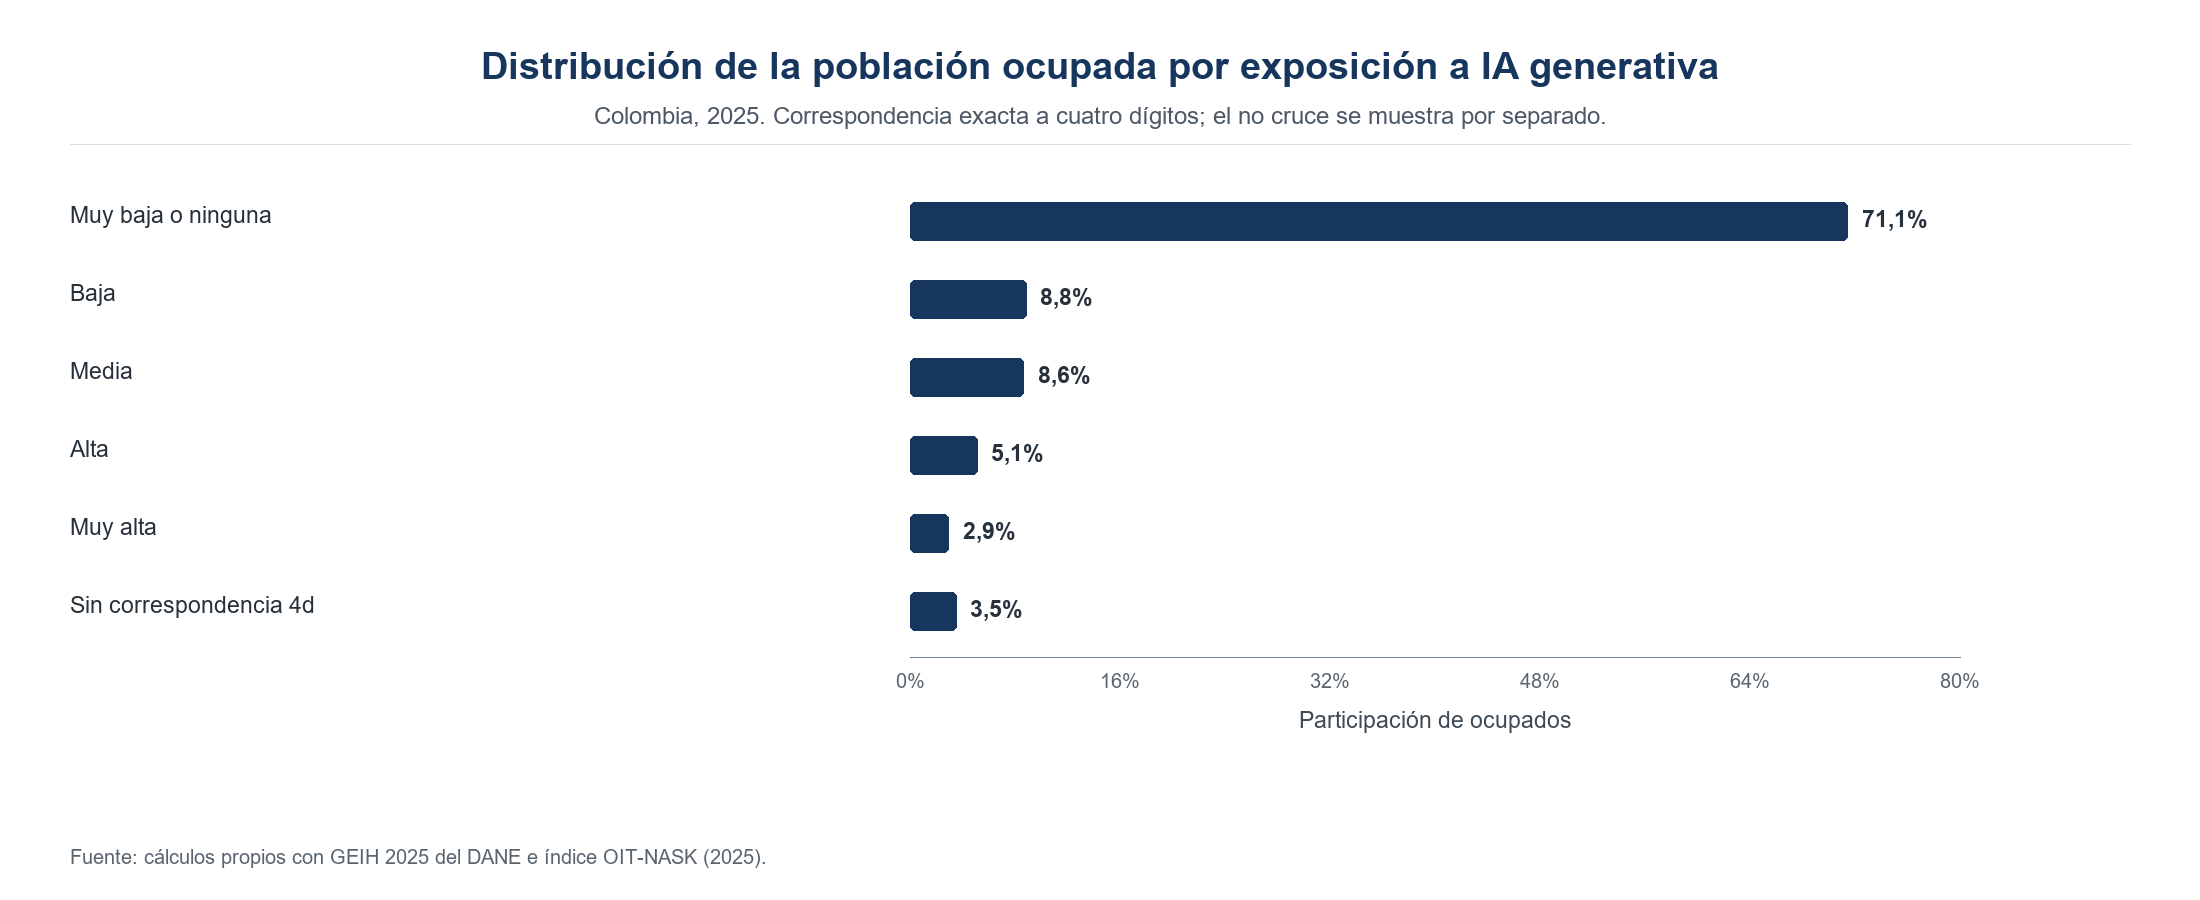
\includegraphics[width=\textwidth]{figures/fig_01_distribucion_exposicion.png}
\caption{Distribución de los ocupados por nivel de exposición}
\label{fig:distribucion_exposicion}
\end{figure}

La exposición alta o muy alta se concentra, entonces, en una fracción específica del empleo. Más que anticipar la desaparición de puestos completos, el resultado señala dónde existe un mayor margen para que cambie la combinación de tareas que hoy realizan los trabajadores.

\subsection*{La exposición aumenta con el ingreso y la educación}

El gradiente por ingreso es claro. Los dos primeros quintiles registran puntajes cercanos a 0,21, mientras que el quinto alcanza 0,358. El patrón educativo es similar: la exposición pasa de 0,179 entre trabajadores con educación básica primaria a 0,361 entre quienes tienen educación superior o universitaria.

\begin{figure}[H]
\centering
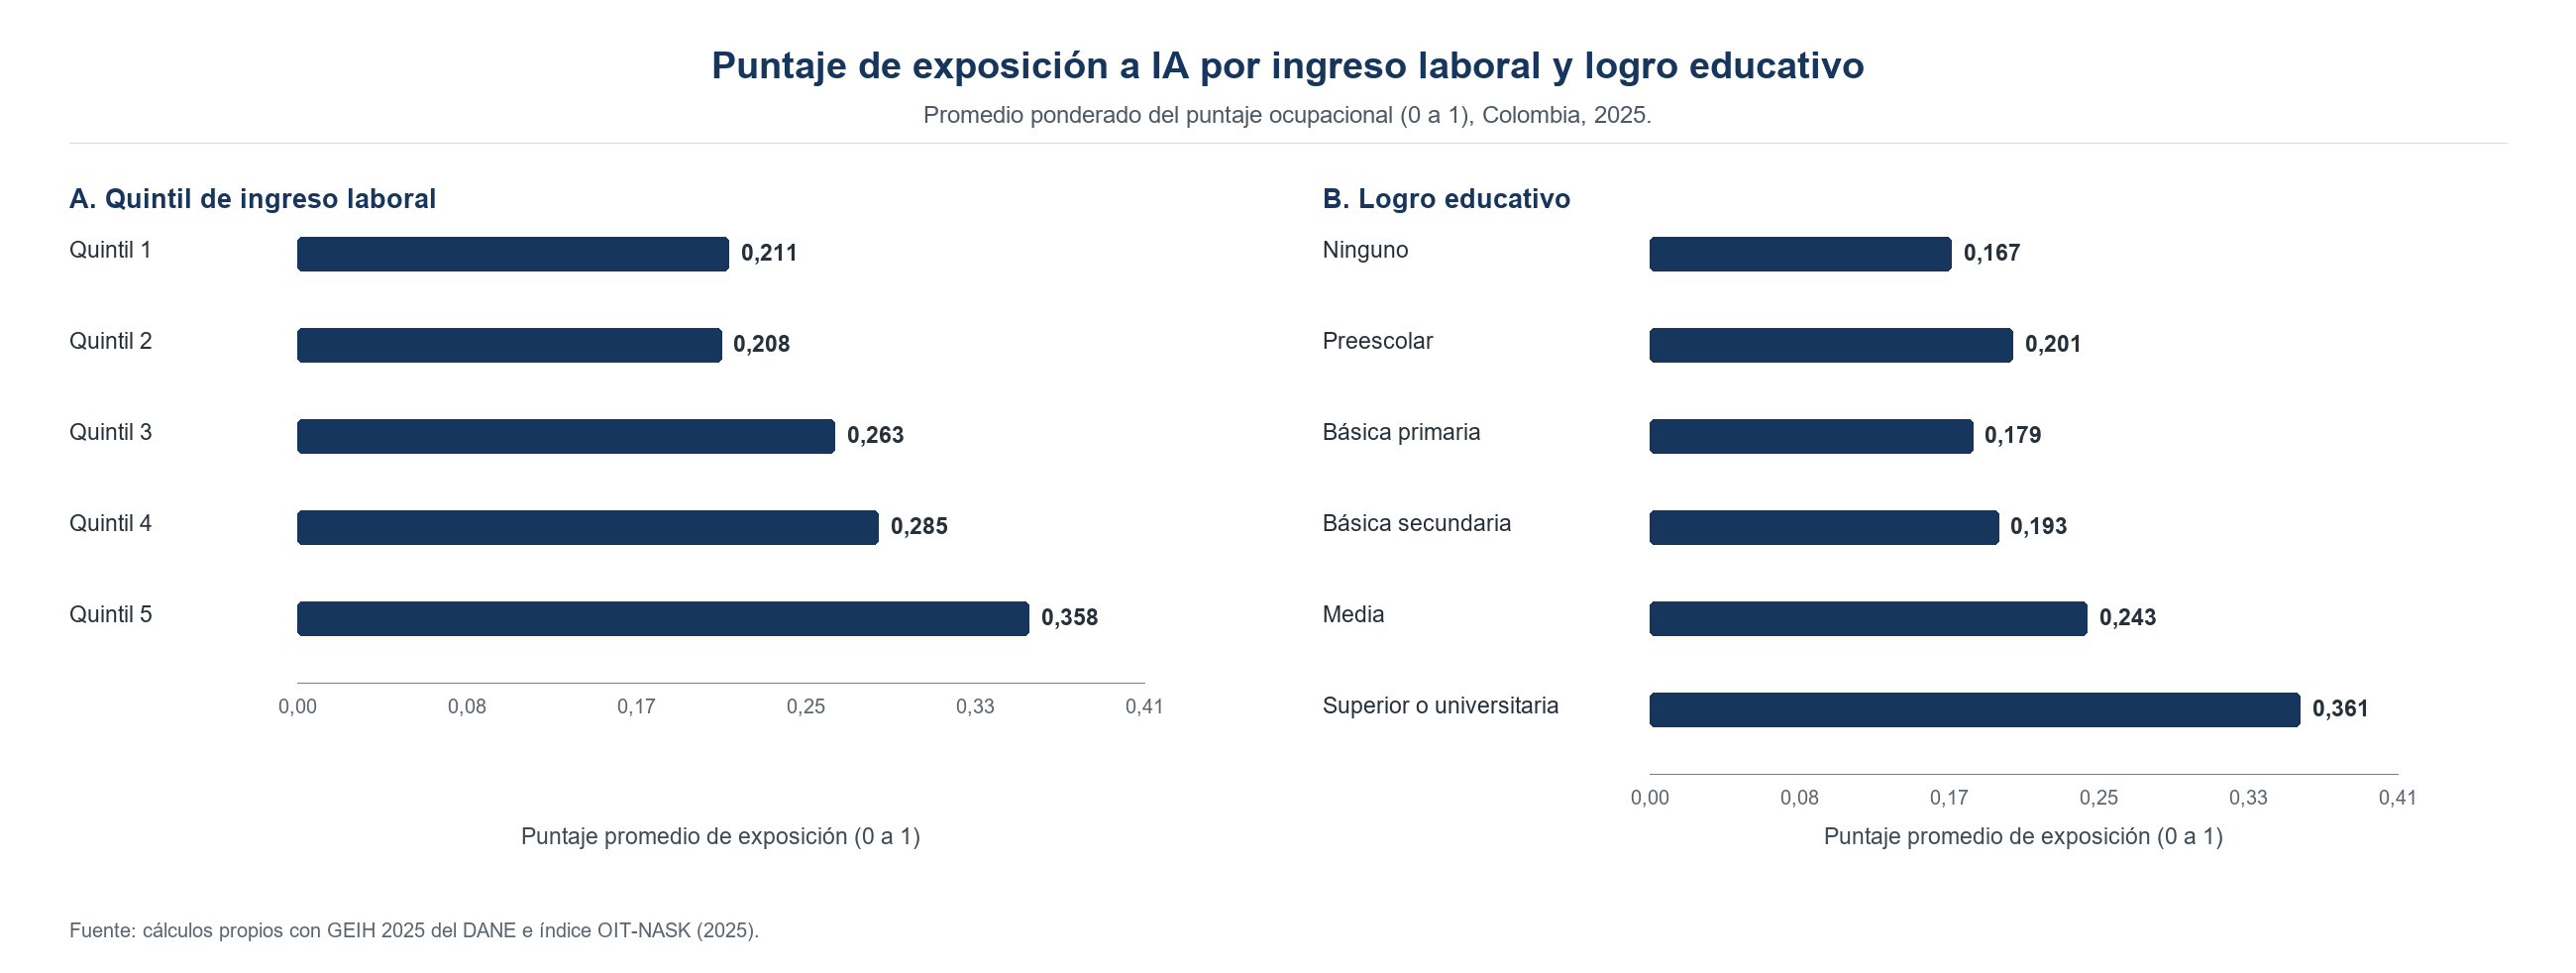
\includegraphics[width=\textwidth]{figures/fig_14_panel_ingreso_educacion.png}
\caption{Puntaje promedio de exposición por quintil de ingreso y logro educativo}
\label{fig:quintiles_ingreso}
\end{figure}

La composición de las tareas ayuda a explicar este patrón. El procesamiento de información, la escritura, el análisis, la programación y la elaboración de documentos tienen mayor peso en ocupaciones profesionales y de oficina, que a su vez se concentran entre trabajadores de mayores ingresos y educación.

\subsection*{Mujeres y trabajadores formales presentan mayor exposición}

La exposición promedio también varía por género y formalidad. El puntaje alcanza 0,297 entre las mujeres y 0,240 entre los hombres. Entre trabajadores formales es de 0,320, frente a 0,217 entre los informales.

\begin{figure}[H]
\centering
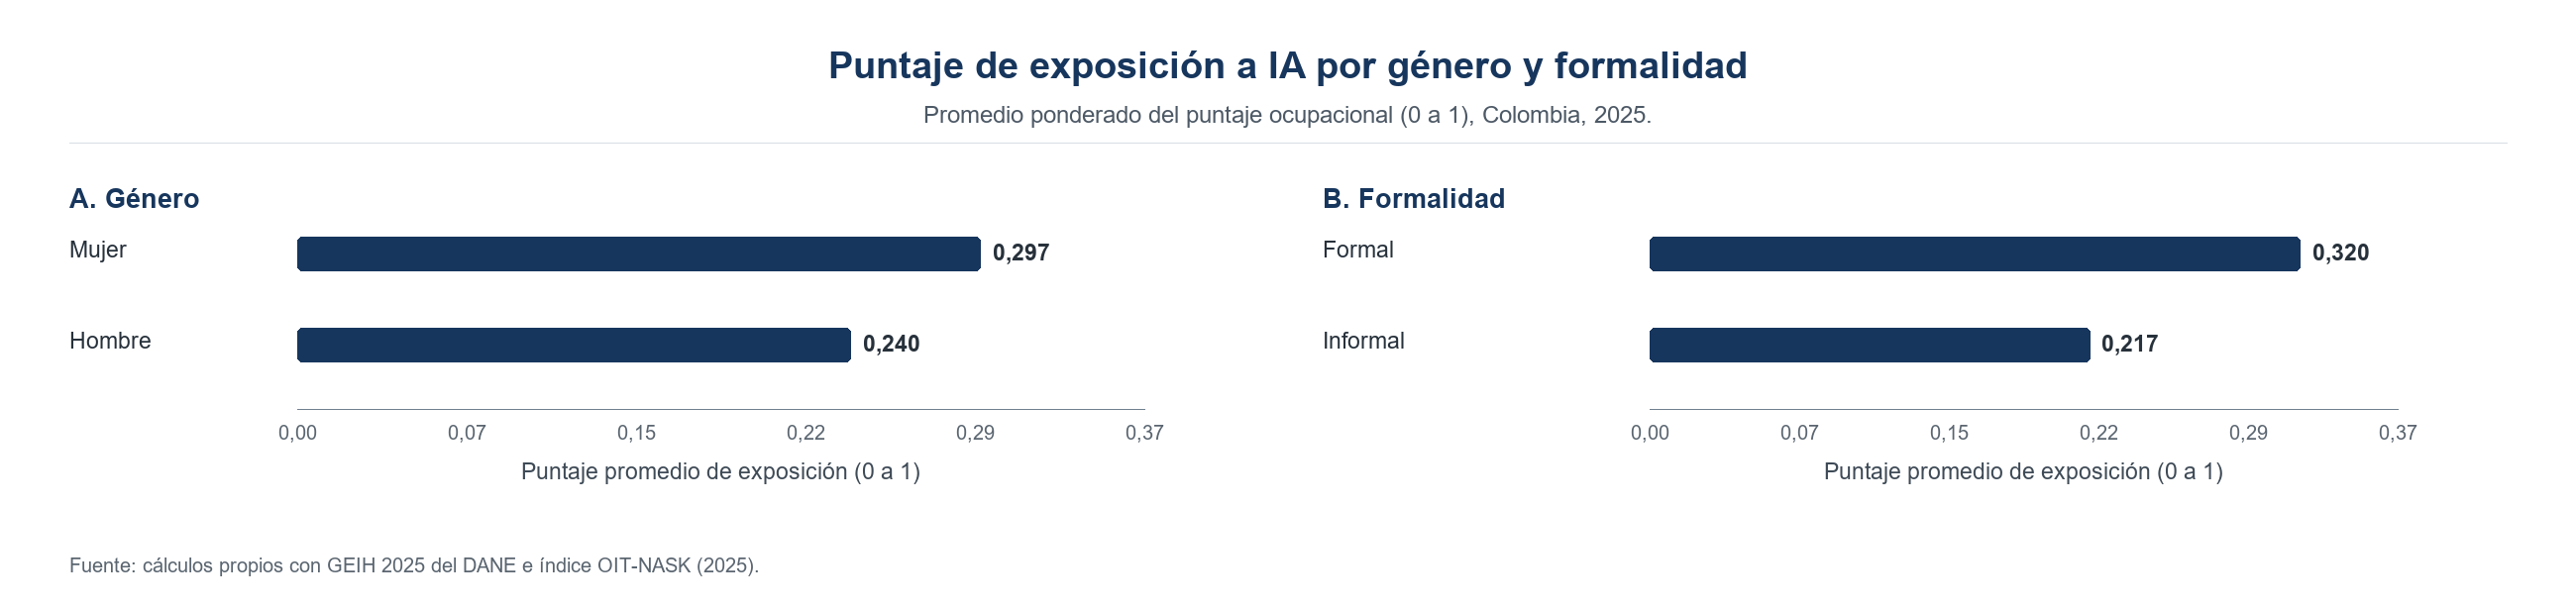
\includegraphics[width=\textwidth]{figures/fig_15_panel_genero_formalidad.png}
\caption{Exposición promedio por género y formalidad}
\label{fig:genero_formalidad}
\end{figure}

Estas diferencias responden en buena medida a la composición ocupacional. Las mujeres tienen una mayor presencia en actividades administrativas, contables y de atención al cliente, mientras que el empleo informal concentra más tareas manuales, presenciales y de servicios personales.

\subsection*{La exposición se concentra en actividades intensivas en información}

Las mayores exposiciones sectoriales aparecen en actividades financieras y de seguros, con un puntaje de 0,478, e información y comunicaciones, con 0,455. En el extremo opuesto, agricultura registra 0,141 y construcción 0,160.

\begin{figure}[H]
\centering
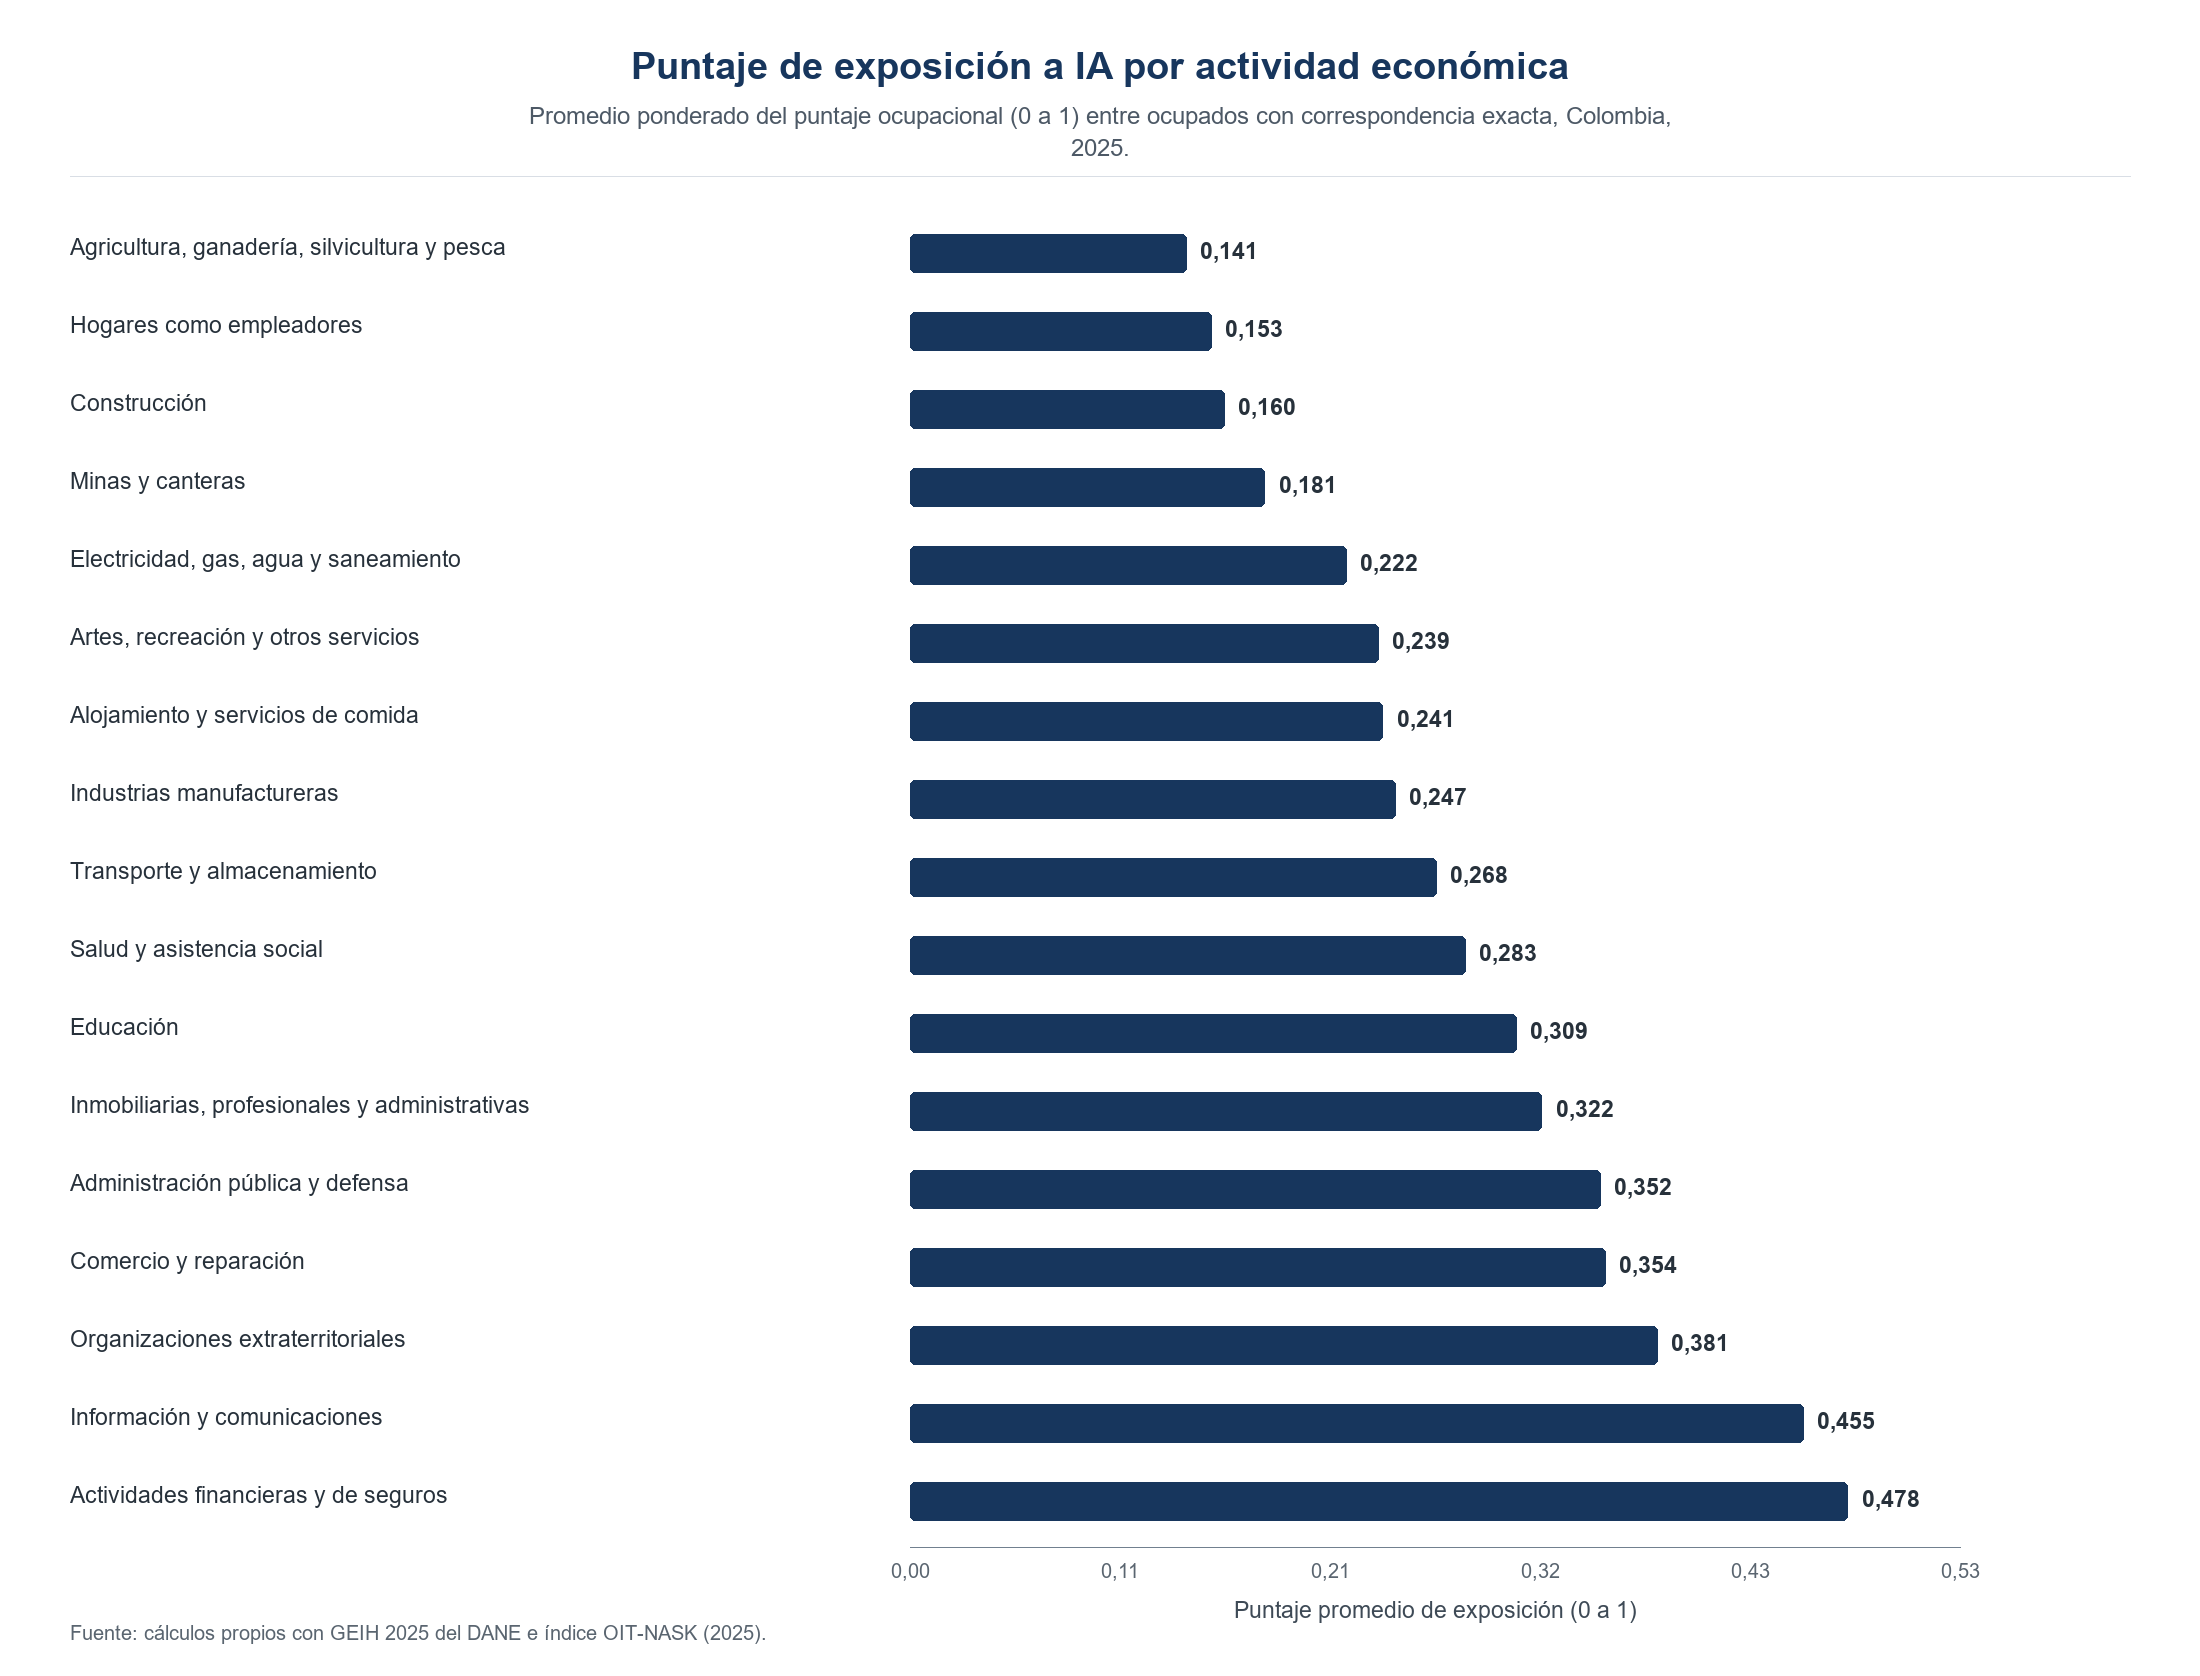
\includegraphics[width=\textwidth,height=0.80\textheight,keepaspectratio]{figures/fig_05_actividad_economica.png}
\caption{Exposición promedio por actividad económica}
\label{fig:actividad_economica}
\end{figure}

El patrón sectorial vuelve a reflejar la naturaleza de las tareas. Las actividades intensivas en procesamiento de información, comunicación, elaboración de documentos y análisis de datos concentran una mayor proporción de funciones compatibles con la inteligencia artificial generativa. Los bajos valores de agricultura o construcción se refieren únicamente a este tipo de tecnología y no a otras formas de automatización.

Las diferencias territoriales siguen una lógica semejante. Bogotá presenta el mayor puntaje promedio, seguida por Antioquia, Atlántico y Valle del Cauca, territorios con una mayor concentración de servicios profesionales, administrativos y tecnológicos.

\begin{figure}[H]
\centering
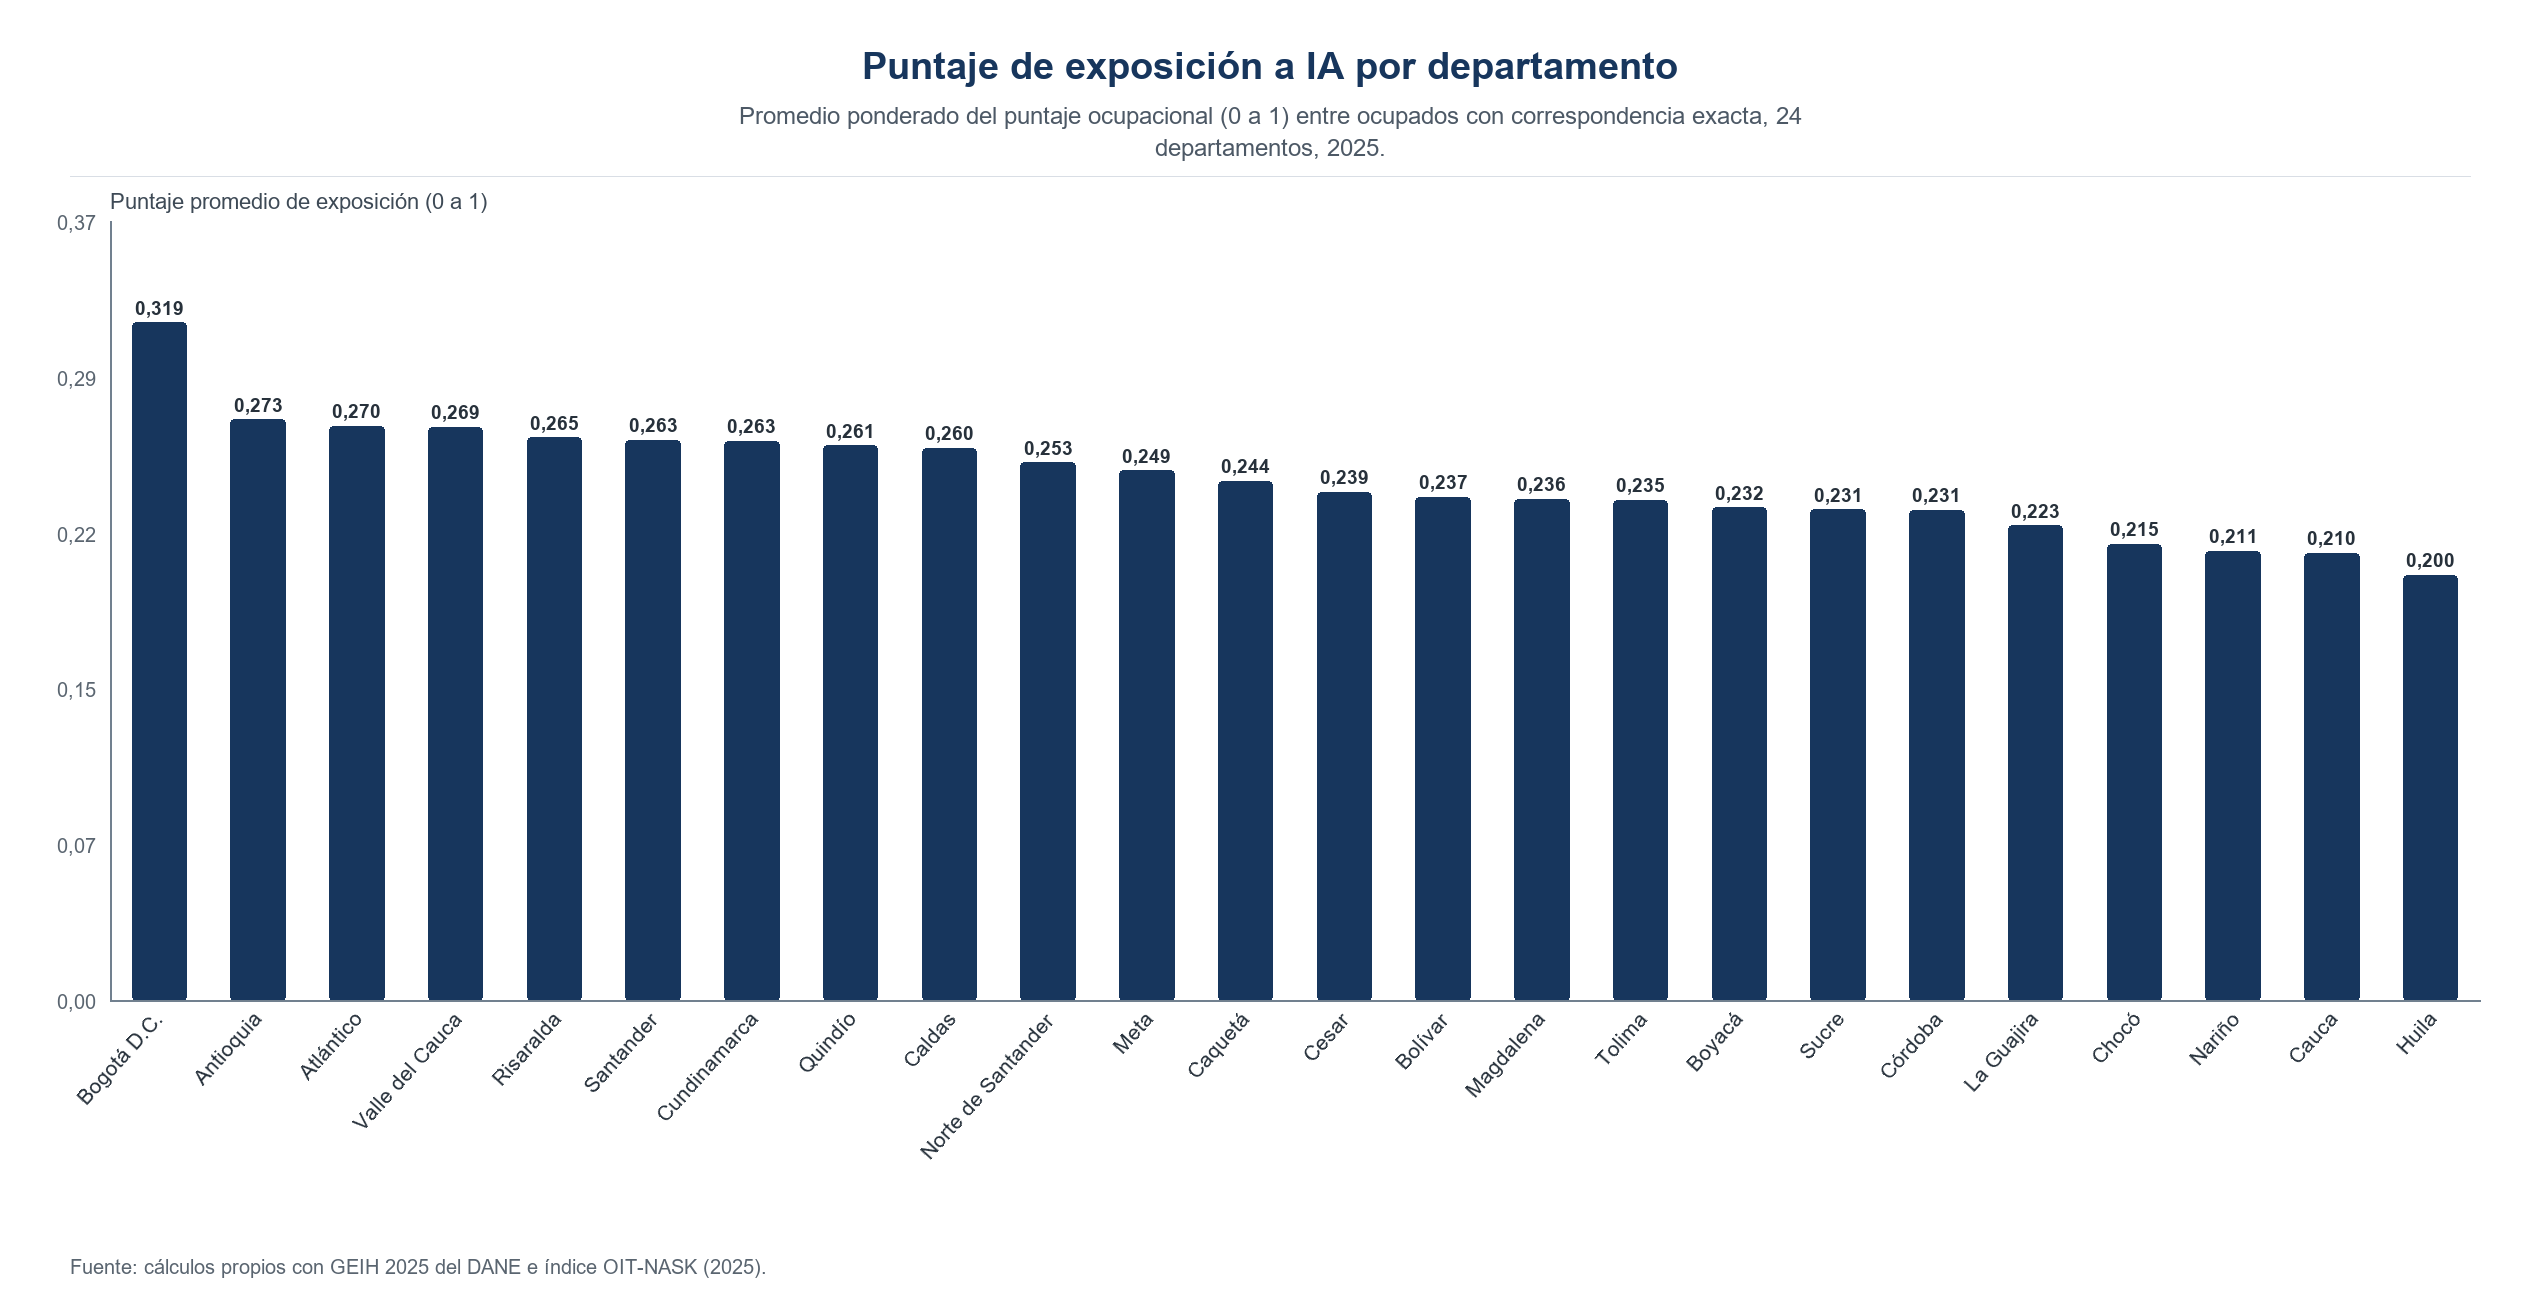
\includegraphics[width=\textwidth,height=0.78\textheight,keepaspectratio]{figures/fig_04_departamentos.png}
\caption{Puntaje promedio de exposición por departamentos}
\label{fig:departamentos}
\end{figure}

\subsection*{Las ocupaciones más expuestas se concentran en oficina, contabilidad y servicios digitales}

Entre las ocupaciones de exposición alta o muy alta con mayor peso en el empleo se encuentran oficinistas generales, contadores, empleados de centros de llamadas, auxiliares de contabilidad y cálculo de costos, secretarios generales y desarrolladores de software.

\begin{figure}[H]
\centering
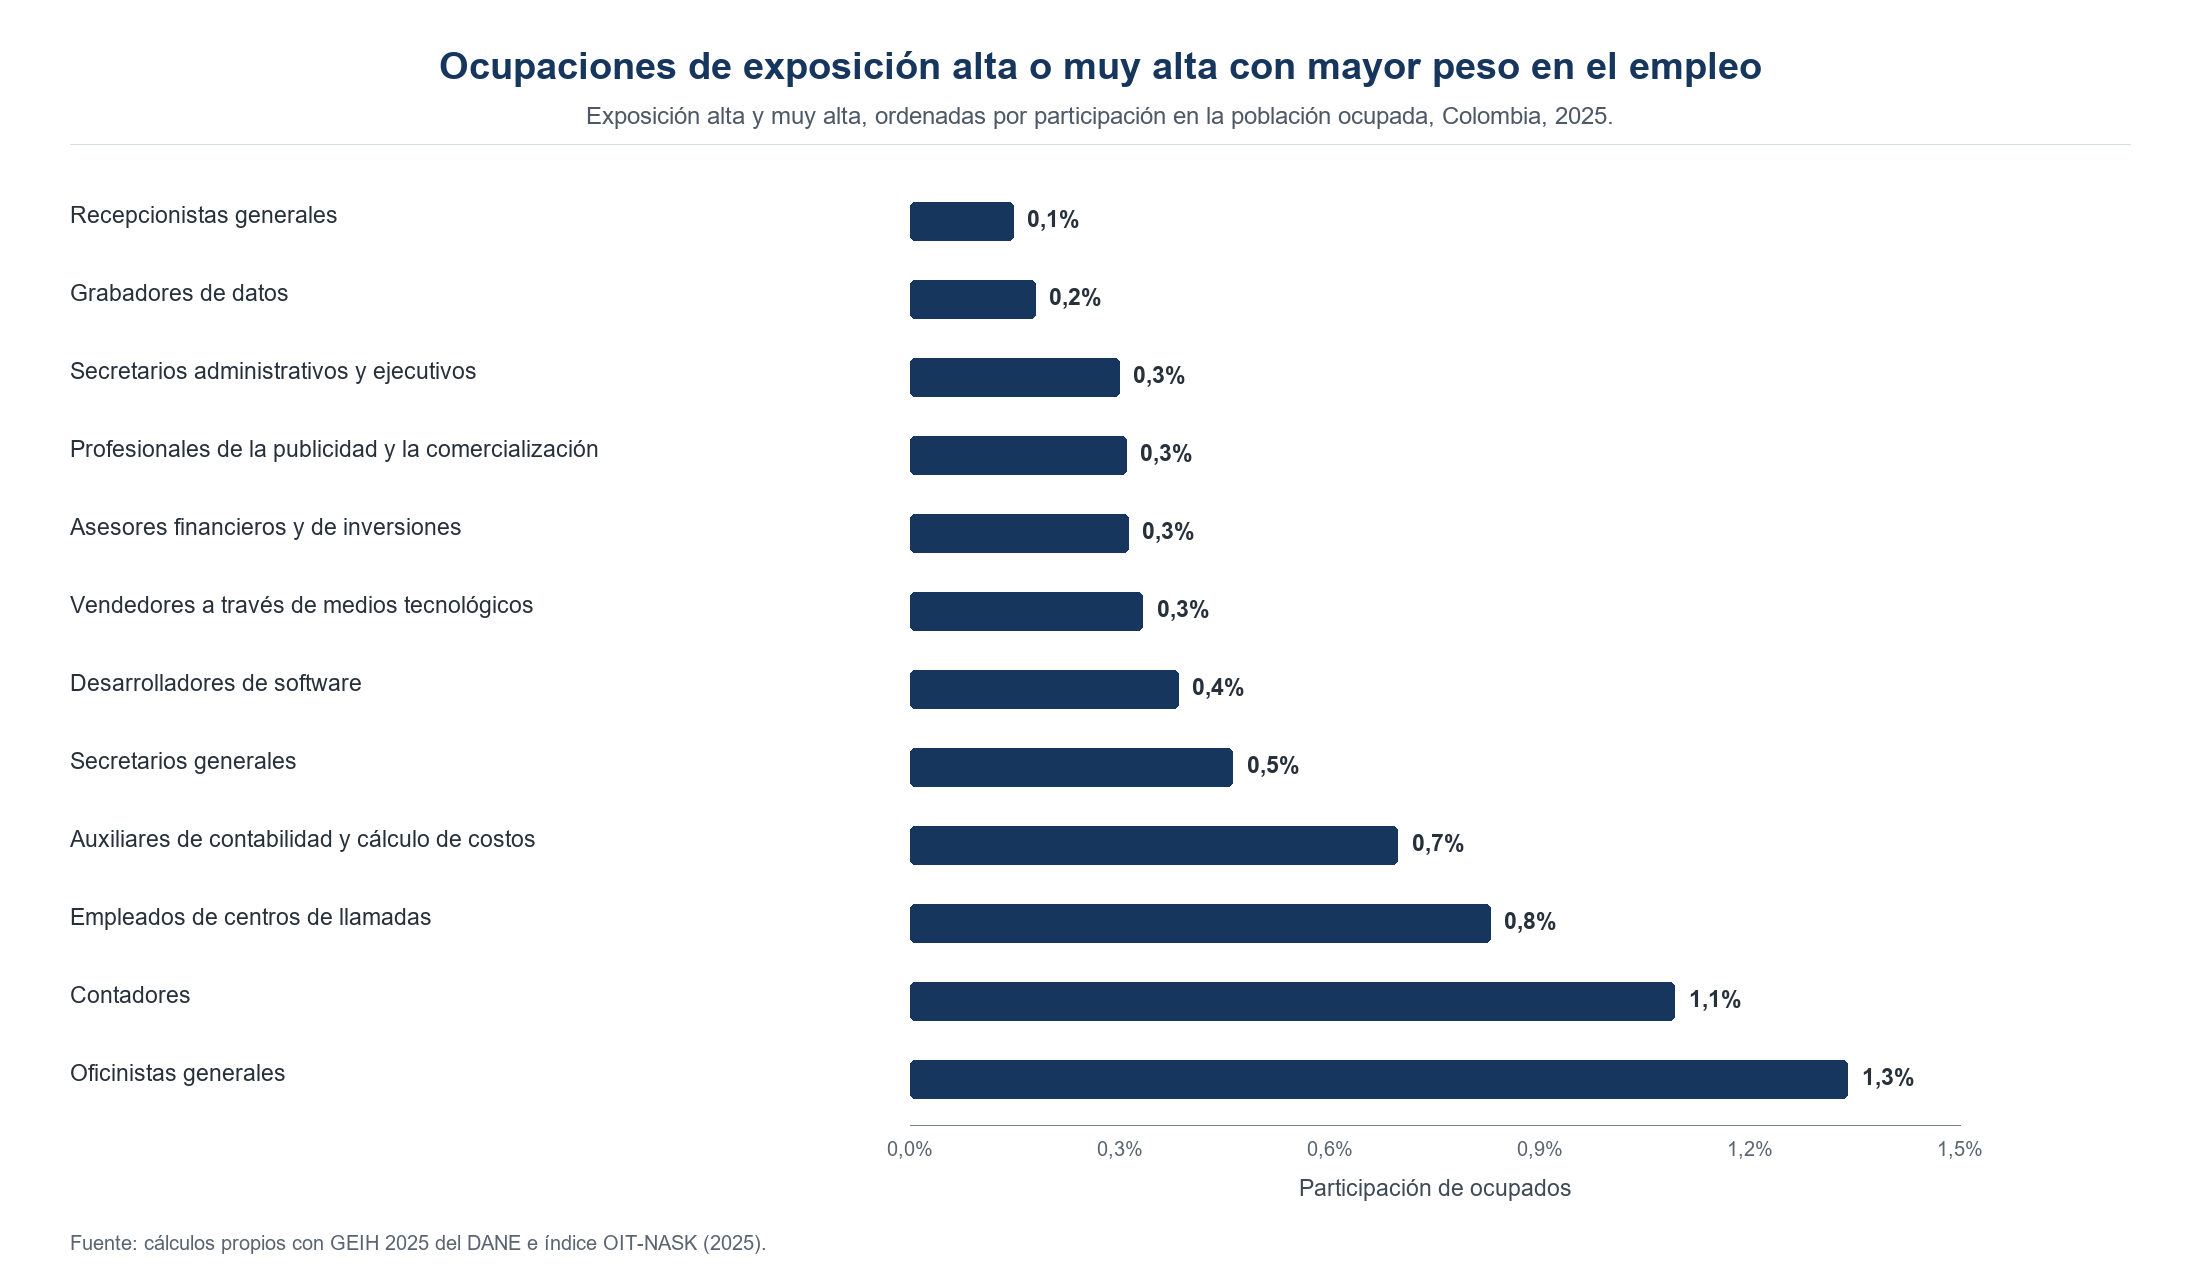
\includegraphics[width=\textwidth]{figures/fig_08_ocupaciones_alta_exposicion.png}
\caption{Ocupaciones de exposición alta o muy alta con mayor peso en el empleo}
\label{fig:ocupaciones_alta_exposicion}
\end{figure}

Estas ocupaciones concentran tareas como registrar información, elaborar documentos, responder solicitudes, clasificar datos, preparar informes, procesar operaciones o producir código. La exposición es alta precisamente porque una parte importante de esas actividades se encuentra cerca de las capacidades actuales de los sistemas generativos.

El siguiente paso es distinguir qué ocurre alrededor de esas tareas: cuánto espacio conserva el trabajador para funciones que requieren juicio, responsabilidad, comunicación o interacción humana.

\section{Exposición no significa sustitución}

Una ocupación altamente expuesta puede combinar automatización de algunas tareas con aumentos de productividad en otras. El resultado depende de las características del puesto y de la importancia que conservan funciones difíciles de delegar completamente a un sistema automatizado.

El ejercicio AIOE/CAIOE permite aproximarse a esta diferencia. En Colombia, el 47,8\% del empleo se ubica en ocupaciones de baja exposición según esta métrica; el 28,3\% combina alta exposición con alta complementariedad potencial y el 20,7\% combina alta exposición con baja complementariedad. El resto corresponde a ocupaciones sin correspondencia.

\begin{figure}[H]
\centering
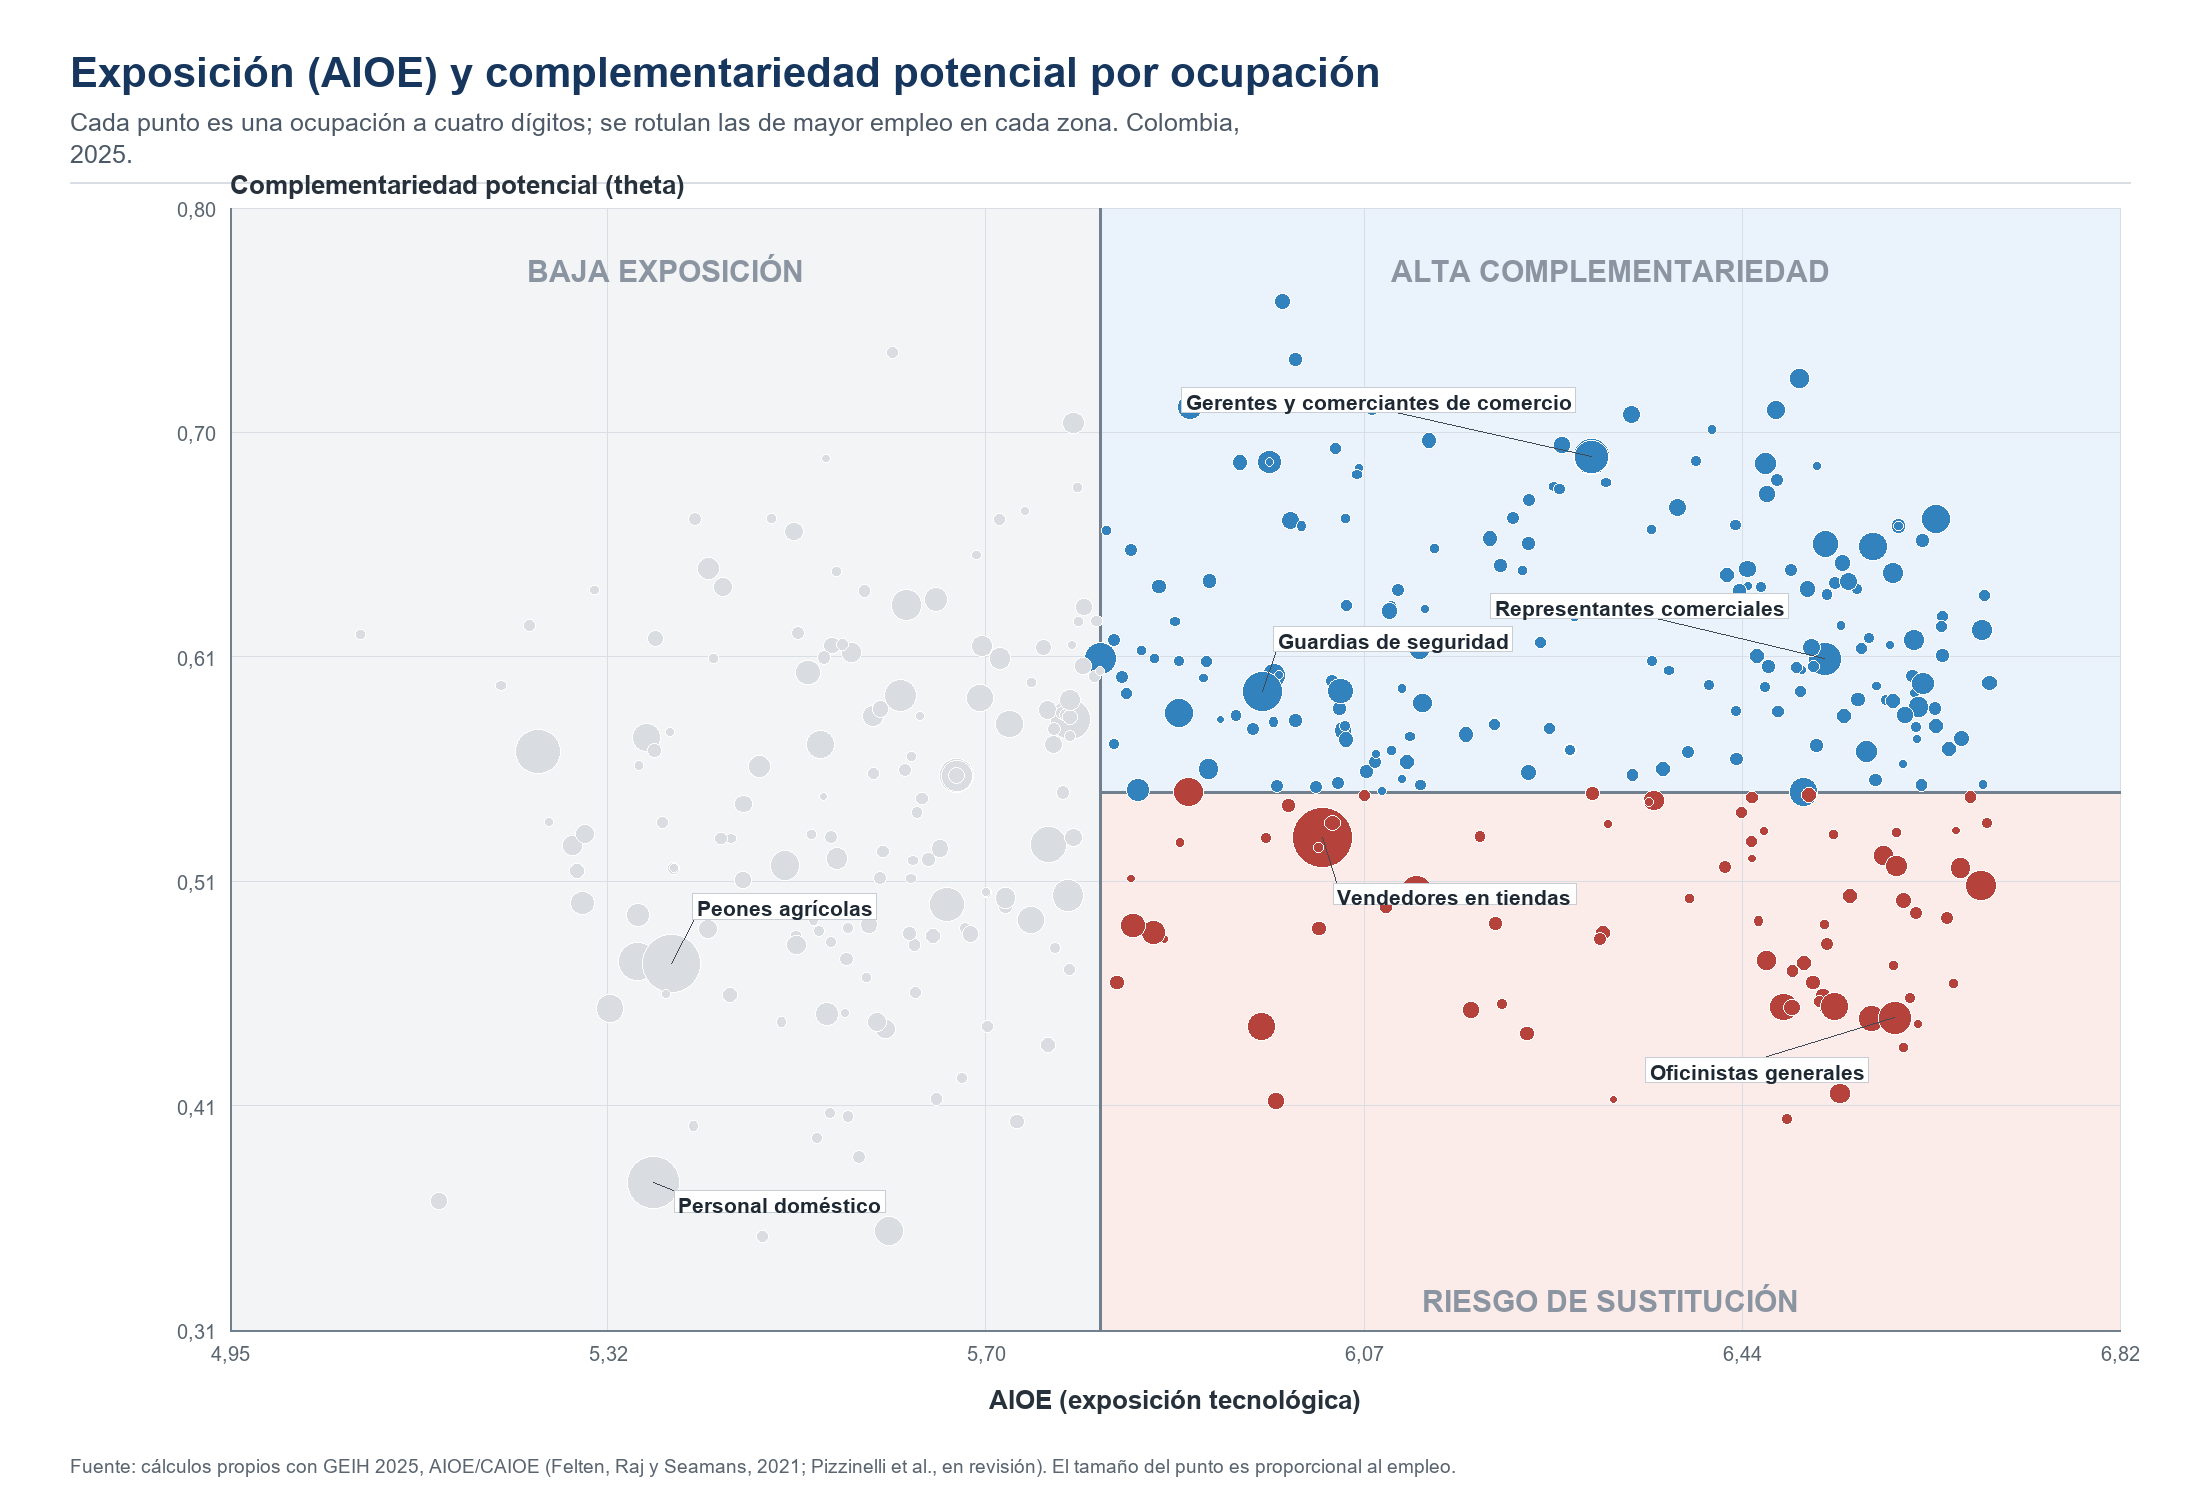
\includegraphics[width=\textwidth,height=0.76\textheight,keepaspectratio]{figures/fig_09_cuadrante_exposicion_complementariedad.png}
\caption{Exposición y complementariedad potencial por ocupación}
\label{fig:cuadrante_exposicion_complementariedad}
\end{figure}

Las ocupaciones expuestas forman grupos muy distintos. Oficinistas, auxiliares contables, cajeros y empleados de centros de llamadas aparecen con mayor frecuencia entre aquellas de baja complementariedad. En contraste, docentes, abogados, gerentes, representantes comerciales y supervisores combinan exposición tecnológica con tareas donde la comunicación, la responsabilidad y el juicio mantienen un peso importante.

\begin{table}[H]
    \centering
    \caption{Ejemplos de ocupaciones según el tipo de exposición a la inteligencia artificial}
    \label{tab:ocupaciones_complementariedad}

    \scriptsize
    \renewcommand{\arraystretch}{1.05}
    \setlength{\tabcolsep}{4pt}

    \begin{tabularx}{\textwidth}{
        >{\raggedright\arraybackslash}X
        >{\raggedright\arraybackslash}X
    }
        \toprule
        \textbf{Alta exposición y baja complementariedad}
        & \textbf{Alta exposición y alta complementariedad} \\

        \textit{Mayor potencial relativo de sustitución de tareas}
        & \textit{Mayor potencial de complementariedad} \\

        \midrule

        Oficinistas generales
        & Profesores de educación secundaria \\

        Contadores
        & Abogados \\

        Empleados de centros de llamadas
        & Representantes comerciales \\

        Auxiliares de contabilidad y cálculo de costos
        & Supervisores de oficina \\

        Cajeros de comercio, taquilleros y expendedores de boletas
        & Gerentes de comercios al por mayor y al por menor \\

        \bottomrule
    \end{tabularx}

    \begin{minipage}{\textwidth}
        \vspace{0.05cm}
        \tiny
        \textit{Nota:} La clasificación corresponde al ejercicio AIOE/CAIOE
        aplicado al empleo colombiano. Las categorías describen características
        potenciales de las ocupaciones y no predicen pérdidas o ganancias de empleo.
    \end{minipage}
\end{table}

La complementariedad tiende a ser mayor cuando el valor del puesto depende de asumir responsabilidad sobre decisiones, interactuar con otras personas, supervisar resultados o resolver excepciones. Estas características ayudan a entender por qué dos ocupaciones cercanas en exposición tecnológica pueden enfrentar trayectorias laborales muy diferentes.

\section{La capacidad de beneficiarse de la inteligencia artificial también es desigual}

\subsection*{Ingresos}

La exposición aumenta con el ingreso. La razón entre empleo en ocupaciones de alta y baja complementariedad aumenta de 0,75 en el primer quintil a 2,80 en el quinto. Hasta el tercer quintil, las ocupaciones de baja complementariedad tienen un mayor peso relativo; en los dos quintiles superiores la relación se invierte.

\begin{figure}[H]
\centering
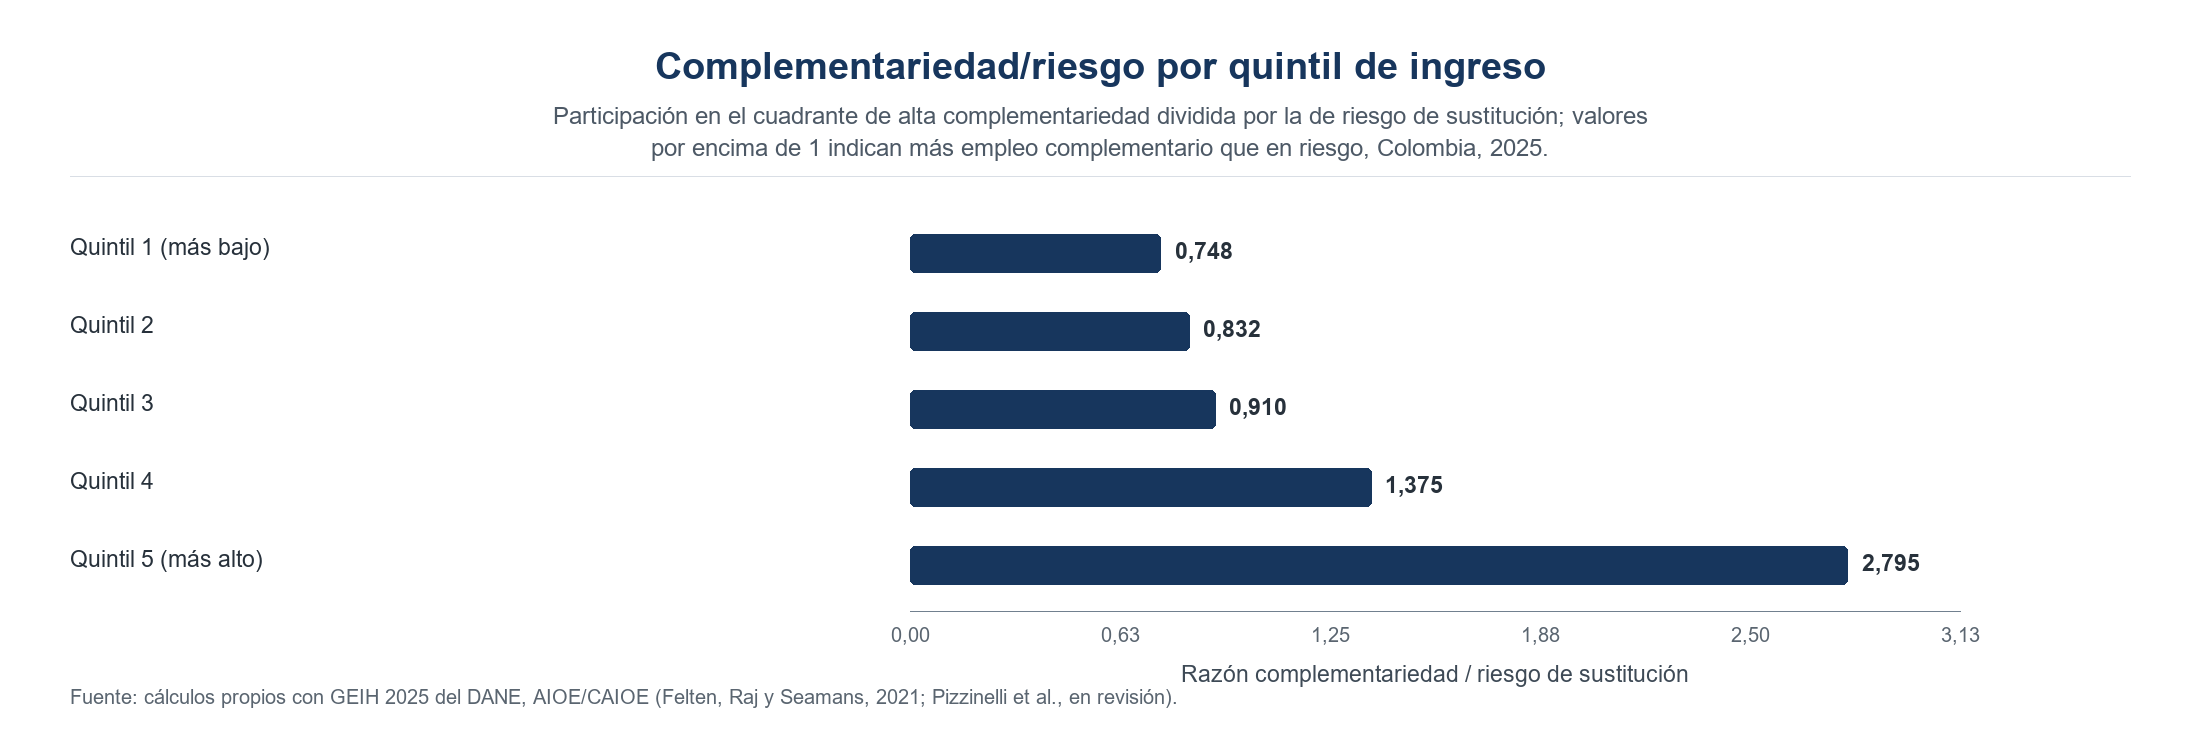
\includegraphics[width=\textwidth,height=0.76\textheight,keepaspectratio]{figures/fig_16_razon_complementariedad_ingreso.png}
\caption{Razón entre complementariedad y baja complementariedad por quintil de ingreso}
\label{fig:razon_complementariedad_ingreso}
\end{figure}

La distribución de los riesgos y oportunidades asociados con la inteligencia artificial no coincide, por tanto, con la distribución de la exposición. Los trabajadores de mayores ingresos aparecen más cerca de la frontera tecnológica, pero también ocupan puestos en los que existen mayores posibilidades de utilizarla como complemento. Entre los trabajadores de menores ingresos la exposición es menor, aunque cuando aparece se concentra relativamente más en ocupaciones de baja complementariedad.

La desigualdad asociada con la inteligencia artificial puede surgir así por una vía distinta a la habitual brecha de acceso tecnológico. Incluso si el uso de estas herramientas se generaliza, las diferencias en las tareas, las habilidades y la organización del trabajo pueden determinar quién logra convertirlas en productividad.

\subsection*{Educación, género y formalidad}

El patrón se repite en otras dimensiones del mercado laboral. La complementariedad relativa aumenta con el nivel educativo: es inferior a uno entre quienes no tienen educación formal y considerablemente mayor entre trabajadores con educación superior. También difiere por género y formalidad. La razón es cercana a uno entre las mujeres y cercana a dos entre los hombres, mientras que alcanza 1,74 entre trabajadores formales y 0,92 entre informales.

\begin{figure}[H]
\centering
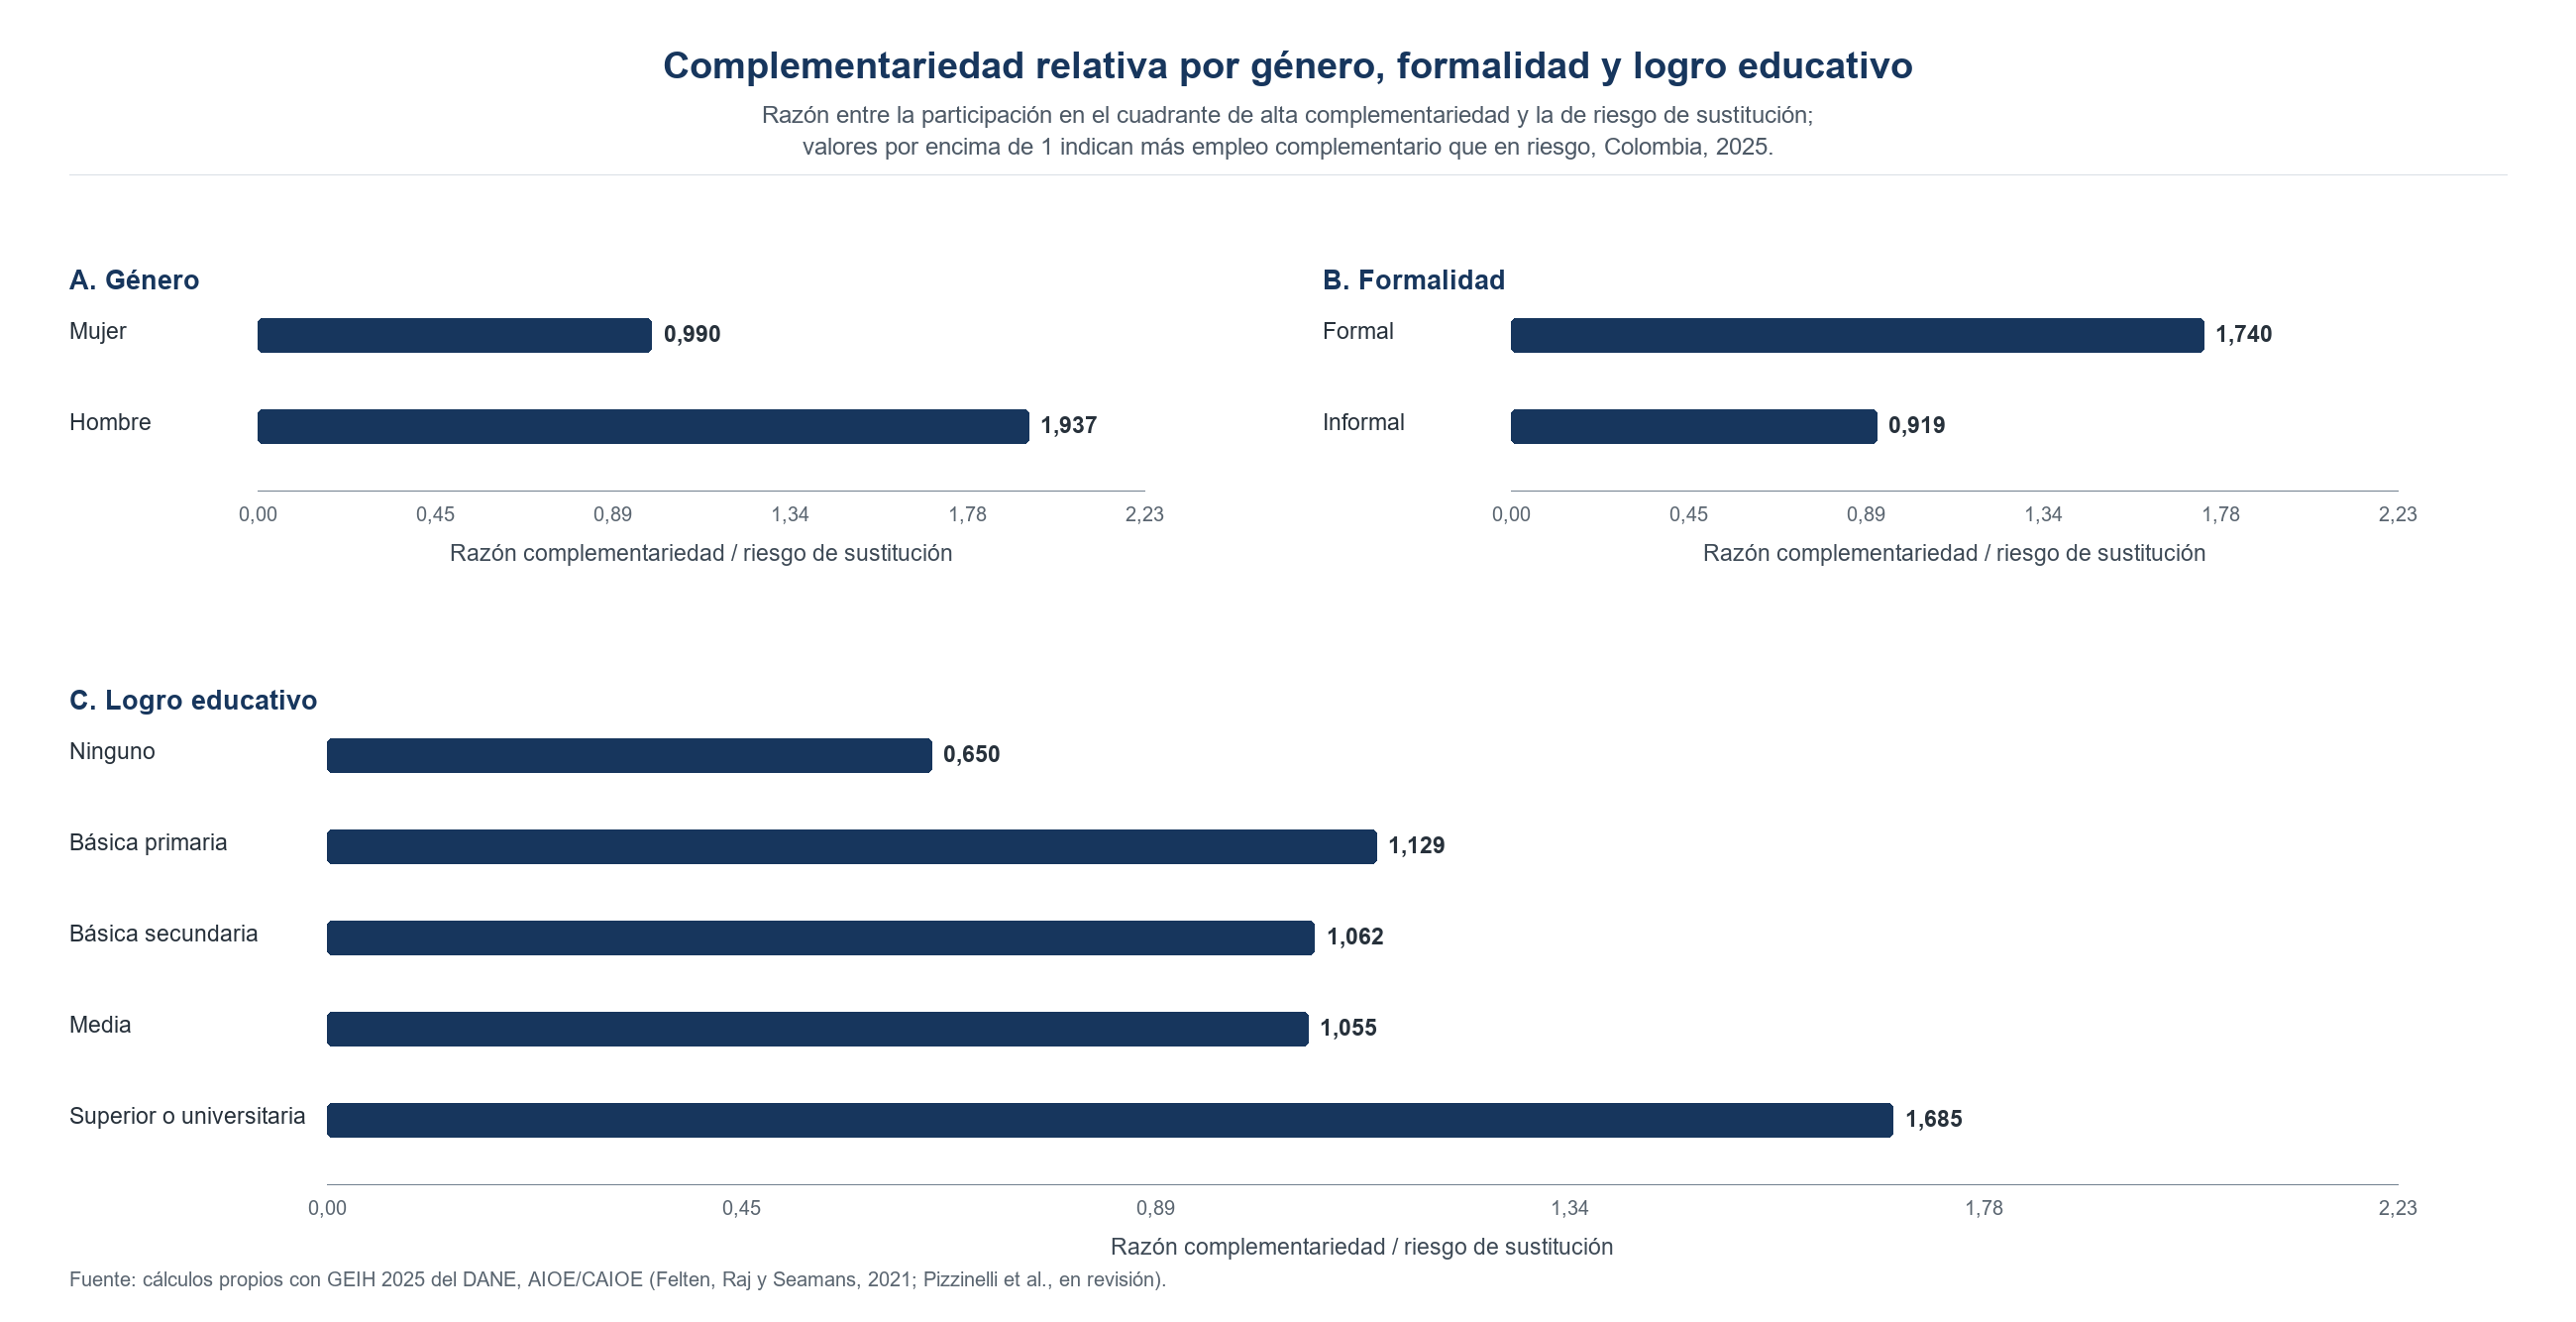
\includegraphics[width=\textwidth,height=0.76\textheight,keepaspectratio]{figures/fig_17_razon_complementariedad_relativa.png}
\caption{Complementariedad relativa por género, formalidad y logro educativo}
\label{fig:razon_complementariedad_relativa}
\end{figure}

La exposición y la capacidad de complementar la tecnología no se distribuyen de la misma manera. Los grupos con mayor ingreso, educación y formalidad pueden estar más expuestos y, al mismo tiempo, relativamente mejor posicionados para capturar las ganancias de productividad. La formación para la transición tecnológica debería considerar ambas dimensiones: cuánto puede cambiar una ocupación y qué margen existe para reorganizar sus tareas alrededor de la nueva tecnología.

\section{¿Qué ocurre cuando la IA se adopta?}

Los indicadores anteriores describen potencial tecnológico. Los efectos económicos comienzan a observarse cuando trabajadores y empresas incorporan efectivamente estas herramientas en sus procesos de producción.

La evidencia disponible sugiere que el primer efecto aparece en la productividad de las tareas. En centros de llamadas, \citet{brynjolfsson2025} estiman un aumento cercano al 15\% en los casos resueltos por hora, con ganancias particularmente altas entre los trabajadores menos experimentados. Un patrón similar aparece en desarrollo de software: \citet{cui2026} documentan un aumento de 26,1\% en las tareas completadas.

Las ganancias dependen, sin embargo, de la naturaleza de la tarea. En actividades de escritura se han documentado mejoras simultáneas en velocidad y calidad \citep{noy2023}. En consultoría, el desempeño aumentó cuando los trabajadores utilizaron inteligencia artificial dentro de la frontera de capacidades de la herramienta, pero se deterioró cuando los problemas excedían esa frontera \citep{dellacqua2026}. Saber cuándo utilizar la tecnología y cómo verificar sus resultados forma parte, por tanto, del proceso de complementariedad.

El aumento de productividad tampoco determina la trayectoria del empleo. En mercados donde una misma producción puede alcanzarse con menos horas de trabajo, las ganancias de eficiencia pueden reducir la demanda por determinadas tareas. \citet{hui2024} documentan este mecanismo entre trabajadores independientes en servicios altamente expuestos, donde la difusión de herramientas generativas estuvo acompañada por caídas en empleo e ingresos.

La evidencia disponible apunta así a una relación menos mecánica que la habitual discusión sobre automatización. La inteligencia artificial puede elevar la productividad y, al mismo tiempo, modificar la demanda de trabajo. La dirección final depende de cómo cambien las tareas, de la capacidad de los trabajadores para complementar la tecnología y de si las ganancias de eficiencia se traducen en mayor producción o en una menor utilización de trabajo.

\section{Implicaciones para Colombia}

Los resultados del informe desplazan la discusión desde la cantidad de empleos expuestos hacia las condiciones que determinan cómo se utiliza la tecnología. Exposición, complementariedad y capacidad de transición describen problemas distintos y requieren respuestas diferentes.

\begin{figure}[H]
    \centering

    \resizebox{0.92\textwidth}{!}{%
    \begin{tikzpicture}[
        node distance=0.3cm,
        every node/.style={
            font=\footnotesize,
            align=center
        },
        main/.style={
            rectangle,
            rounded corners=2pt,
            draw,
            minimum width=2.2cm,
            minimum height=0.9cm,
            inner sep=2pt
        },
        outcome/.style={
            rectangle,
            rounded corners=3pt,
            draw,
            minimum width=2.8cm,
            minimum height=0.8cm,
            inner sep=5pt
        },
        factor/.style={
            rectangle,
            rounded corners=2pt,
            draw,
            dashed,
            minimum width=3.1cm,
            minimum height=0.7cm,
            inner sep=4pt,
            font=\footnotesize
        },
        arrow/.style={
            -{Latex[length=2mm]},
            thick
        },
        factorarrow/.style={
            -{Latex[length=2mm]},
            dashed
        }
    ]

    % Cadena principal

    \node[main] (capacity)
    {\textbf{Capacidades de la inteligencia artificial}\\
    Tareas que la tecnología puede realizar o transformar};

    \node[main, below=of capacity] (exposure)
    {\textbf{Exposición ocupacional}\\
    Presencia de esas tareas dentro de cada ocupación};

    \node[main, below=of exposure] (adoption)
    {\textbf{Adopción de inteligencia artificial}\\
    Uso efectivo por empresas y trabajadores};

    \node[main, below=of adoption] (reorganization)
    {\textbf{Reorganización del trabajo}\\
    Cambio en la combinación y distribución de tareas};

    % Automatización y complementariedad

    \node[outcome, below left=0.9cm and 0.5cm of reorganization]
    (automation)
    {\textbf{Automatización}\\
    Sustitución de algunas tareas};

    \node[outcome, below right=0.9cm and 0.5cm of reorganization]
    (complement)
    {\textbf{Complementariedad}\\
    IA como apoyo al trabajador};

    % Productividad y calidad

    \node[main, below=2.0cm of reorganization] (productivity)
    {\textbf{Productividad y calidad}\\
    Cambios en tiempo, producción, errores y desempeño};

    % Resultados laborales finales

    \node[outcome, below left=0.9cm and 1.4cm of productivity]
    (employment)
    {\textbf{Empleo}\\
    Demanda de trabajo};

    \node[outcome, below=0.9cm of productivity]
    (wages)
    {\textbf{Salarios}\\
    e ingresos};

    \node[outcome, below right=0.9cm and 1.4cm of productivity]
    (transitions)
    {\textbf{Transiciones}\\
    ocupacionales};

    % Flechas principales

    \draw[arrow] (capacity) -- (exposure);
    \draw[arrow] (exposure) -- (adoption);
    \draw[arrow] (adoption) -- (reorganization);

    \draw[arrow] (reorganization) -- (automation);
    \draw[arrow] (reorganization) -- (complement);

    \draw[arrow] (automation) -- (productivity);
    \draw[arrow] (complement) -- (productivity);

    \draw[arrow] (productivity) -- (employment);
    \draw[arrow] (productivity) -- (wages);
    \draw[arrow] (productivity) -- (transitions);

    % Factores que condicionan la relación

    \node[factor, left=1.4cm of adoption] (skills)
    {\textbf{Habilidades}\\
    Formación y capacidad de uso};

    \node[factor, right=1.4cm of adoption] (organization)
    {\textbf{Organización empresarial}\\
    Procesos y gestión};

    \node[factor, left=1.4cm of reorganization] (investment)
    {\textbf{Inversión complementaria}\\
    Tecnología e infraestructura};

    \node[factor, right=1.4cm of reorganization] (demand)
    {\textbf{Demanda}\\
    Bienes y servicios};

    \node[factor, right=1.4cm of productivity] (regulation)
    {\textbf{Regulación y entorno institucional}};

    % Flechas de factores

    \draw[factorarrow] (skills) -- (adoption);
    \draw[factorarrow] (organization) -- (adoption);
    \draw[factorarrow] (investment) -- (reorganization);
    \draw[factorarrow] (demand) -- (reorganization);
    \draw[factorarrow] (regulation) -- (productivity);

    \end{tikzpicture}%
    }

    \caption{Cómo la exposición a la inteligencia artificial puede traducirse en resultados laborales}
    \label{fig:mecanismo_ia_empleo}

    \begin{minipage}{0.95\textwidth}
        \vspace{0.2cm}
        \footnotesize
        \textit{Nota:} La exposición tecnológica no determina directamente los
        efectos sobre empleo o salarios. Los resultados dependen de la adopción,
        la reorganización de las tareas, el grado de automatización o
        complementariedad y de factores como las habilidades de los trabajadores,
        la organización empresarial, la inversión complementaria, la demanda y
        el entorno institucional.
    \end{minipage}

\end{figure}

Para las empresas, la unidad relevante de análisis es la tarea. Identificar qué actividades pueden automatizarse, cuáles requieren supervisión y cuáles pueden aumentar su valor mediante nuevas herramientas permite orientar la adopción hacia mejoras de productividad y calidad. Los pilotos deberían evaluar no solo reducciones de tiempo y costos, sino también errores, satisfacción de clientes, carga de trabajo y capacidad de los trabajadores para asumir funciones de mayor valor agregado.

Para los trabajadores, las habilidades relevantes van más allá del manejo técnico de las herramientas. Verificar resultados, detectar errores, formular problemas, interpretar información, comunicarse con clientes y asumir responsabilidad sobre decisiones son capacidades que pueden aumentar el grado de complementariedad con la tecnología.

Para el Gobierno, identificar las ocupaciones expuestas es apenas el punto de partida. Las políticas de formación deberían prestar especial atención a trabajadores que combinan alta exposición con baja complementariedad y menores posibilidades de transición. El seguimiento del mercado laboral también deberá incorporar información sobre adopción empresarial, vacantes, salarios, horas trabajadas y movilidad ocupacional.

La transformación tiene además una dimensión empresarial. Si las capacidades necesarias para adoptar inteligencia artificial se concentran en firmas grandes y productivas, mientras las mipymes enfrentan restricciones de financiamiento, habilidades o infraestructura digital, la tecnología puede ampliar las brechas de productividad ya existentes entre empresas. Facilitar la adopción y la formación en firmas de menor tamaño es, por ello, parte de la misma agenda de transición.

El objetivo no debería ser contener la exposición tecnológica, sino aumentar la capacidad para aprovecharla. Allí donde la inteligencia artificial pueda complementar el trabajo, el reto es acelerar la adopción productiva; donde la sustitución de tareas tenga mayor peso, la prioridad pasa por facilitar la adaptación y la movilidad de los trabajadores.

\section{Conclusiones}

La expansión de la inteligencia artificial generativa no está llegando primero a los trabajadores tradicionalmente asociados con la automatización. En Colombia, la exposición se concentra en ocupaciones administrativas, profesionales y de servicios intensivos en información, y aumenta con el ingreso y la educación. La transformación tecnológica alcanza así una parte del mercado laboral que durante otras olas de automatización estuvo relativamente menos expuesta.

Pero la exposición cuenta solo una parte de la historia. Entre los trabajadores de mayores ingresos y educación también es más frecuente encontrar ocupaciones donde la tecnología puede complementar tareas que requieren juicio, comunicación o responsabilidad. En otros segmentos del mercado laboral, una exposición menor puede estar acompañada por menos espacio para esa complementariedad. La distribución de las oportunidades de productividad no coincide necesariamente con la distribución de la exposición.

Esta diferencia debería orientar la respuesta de empresas y política pública. La prioridad no es proteger ocupaciones de cualquier contacto con la inteligencia artificial, sino ampliar las capacidades para reorganizar el trabajo alrededor de ella y facilitar las transiciones donde la sustitución de tareas sea más probable. La pregunta relevante para Colombia no es únicamente qué trabajos puede transformar la tecnología, sino quién estará en condiciones de aprovechar esa transformación.

\section*{Reproducibilidad}

El programa \texttt{code/01\_analisis\_exposicion\_ia\_2025.py} genera las tablas CSV, las figuras base y las pruebas de calidad. Los insumos principales son \texttt{BaseIA.dta}, la correlativa CIUO-08/GEIH y el archivo público de tareas de la OIT. Ningún resultado del informe usa la imputación a dos dígitos como estimación principal.

\bibliographystyle{apalike}
\bibliography{references}

\end{document}
